\chapter{RESULTS}
\label{ch:results}

This chapter is divided into two sections. The first section focuses on the comparison of the two motion correction techniques. The second section focuses on the results of the machine learning algorithms applied to the metrics extracted from the images.

\section{Volume Registration} 

Each of the clinical images underwent volume registration using both registration methods outlined in Chapter \ref{ch:moco}. The FD and DVARs metrics were calculated for every pair of subsequent volumes $i$ and $i+1$ in the original sequences, the traditionally registered sequences, and the DAG-registered sequences. 

The FD and DVARS values for each sequence were compared to the usability thresholds established by Power et al. \cite{Power2012}. These thresholds state that an image sequence is usable if at least 50\% of the image volumes within it have FD $<$ 2.0 mm and DVARS $<$ 2.5\% signal intensity change. The counts of image volumes which met these thresholds were calculated for each sequence type.

A series of independent two-sample t-tests were performed to determine the statistical significance of the differences in the counts of image volumes meeting each threshold. Three comparison pairs were used: the original sequence and the traditionally registered sequence, the original sequence and the DAG-registered sequence, and the two registered sequence types. The distributions of samples were the numbers of image volumes in each sequence meeting the usability threshold of interest. The null hypothesis of the t-tests was that the number of image volumes meeting the threshold being tested was the same for both sequence types.

The FD and DVARS metrics measure motion with respect to a pair of usability standards, but they offer a limited perspective about the motion present throughout an image sequence. Motion across the entire image was measured by calculating a similarity metric between every image volume $i$ and every other image volume $j$. 

Motion across the whole sequence was measured by comparing every image volume in the sequence to every other image volume in the same sequence. The three metrics used for this comparison were the Dice metric and mutual information (MI). The calculations for a single metric on one sequence produce a two-dimensional matrix of metric values. These matrices were used to compare the quantities of motion throughout an entire sequence. 

To describe the distribution of the similarity metrics matrices for the original sequence and each registered sequence, the minimum, first quartile, median, third quartile, and maximum values of each matrix were computed. The distributions of these five values were compared between registration types using two-sample t-tests.

The distributions of all matrix values for the same similarity metric were compared using the Kolmogorov-Smirnov test. Three Kolmogorov-Smirnov tests were performed to compare the distributions of each metric for the original and traditionally registered sequences, the original and DAG-registered sequences, and the traditionally registered and DAG-registered sequences.

The simulated data underwent the same analyses as the clinical images, with one addition. Independent component analysis was performed on the simulated data to identify the signal components which contribute to the overall signal in the image. By correlating the components for each image with the DMN ROIs, the BOLD-related components were identified. The BOLD-related components were compared to the DMN ROIs on a voxel level to determine how many signal related voxels in the components were correctly recovered by the registrations.

For brevity, several tables of p-values have been moved to Appendix \ref{appendix:results} but are summarized here.

\subsection{Simulated Data}

\subsubsection{Volume Registration: Power Thresholds}

\begin{figure}[]
	\centering
	\begin{subfigure}{0.4\textwidth}
		\centering
		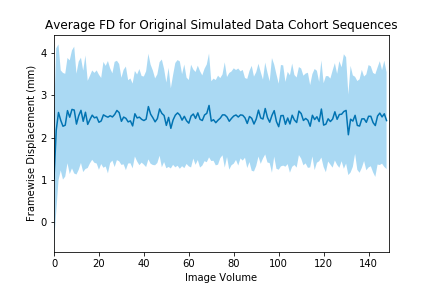
\includegraphics[width=1.0\textwidth]{6/figures/spectr-bold-fd-150.png}
		\caption{FD of Original Sequences.}
	\end{subfigure}
	\hspace{0.05\textwidth}
	\begin{subfigure}{0.4\textwidth}
		\centering
		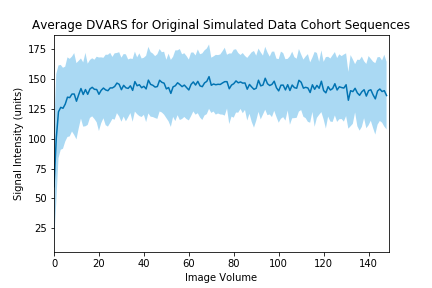
\includegraphics[width=1.0\textwidth]{6/figures/spectr-bold-dvars-150.png}
		\caption{DVARS of Original Sequences.}
	\end{subfigure}
	
	\begin{subfigure}{0.4\textwidth}
		\centering
		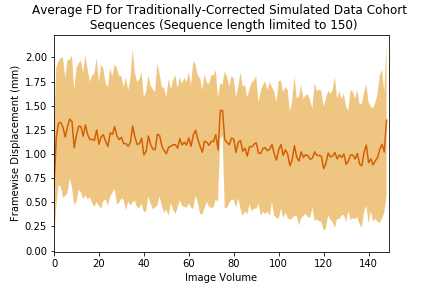
\includegraphics[width=1.0\textwidth]{6/figures/spectr-trad-fd-150.png}
		\caption{FD of Traditionally Registered Sequences.}
	\end{subfigure}
	\hspace{0.05\textwidth}
	\begin{subfigure}{0.4\textwidth}
		\centering
		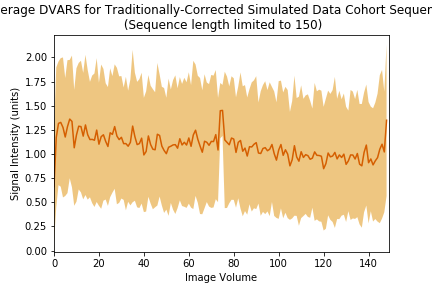
\includegraphics[width=1.0\textwidth]{6/figures/spectr-trad-dvars-150.png}
		\caption{DVARS of Traditionally Registered Sequences.}
	\end{subfigure}
	
	\begin{subfigure}{0.4\textwidth}
		\centering
		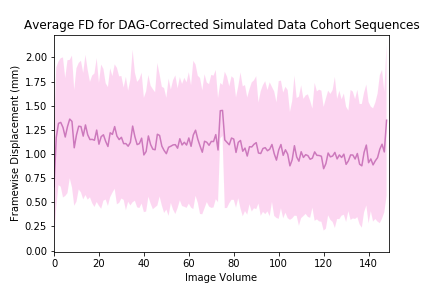
\includegraphics[width=1.0\textwidth]{6/figures/spectr-dag-fd-150.png}
		\caption{FD of DAG-Registered Sequences.}
	\end{subfigure}
	\hspace{0.05\textwidth}
	\begin{subfigure}{0.4\textwidth}
		\centering
		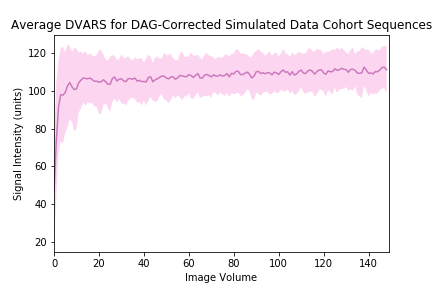
\includegraphics[width=1.0\textwidth]{6/figures/spectr-dag-dvars-150.png}
		\caption{DVARS of DAG-Registered Sequences.}
	\end{subfigure}
\caption{The means and standard deviations of the FD and DVARS metrics for all simulated images before and after each type of registration.}
\label{fig:spectr-power-dists}
\end{figure}

\begin{figure}[]
	\centering	
	\begin{subfigure}{0.4\textwidth}
		\centering
		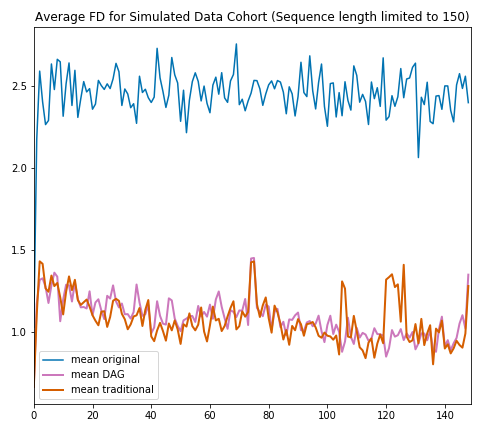
\includegraphics[width=1.0\textwidth]{6/figures/spectr_fd_all_150_avg.png}
		\caption{Average FD}
	\end{subfigure}
	\hspace{0.05\textwidth}
	\begin{subfigure}{0.4\textwidth}
		\centering
		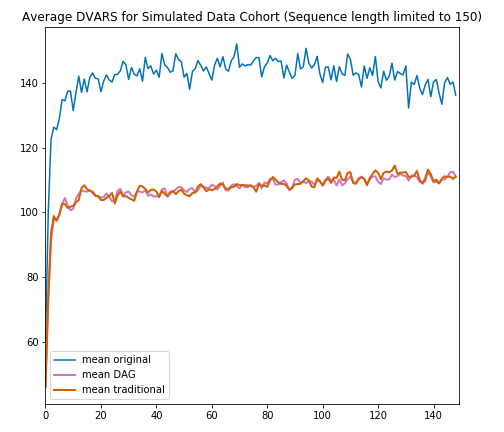
\includegraphics[width=1.0\textwidth]{6/figures/spectr_dvars_all_150_avg.png}
		\caption{Average DVARS}
	\end{subfigure}
\caption{The means of the FD and DVARS metrics for all simulated images before and after both registrations.}
\label{fig:spectr-power-means}
\end{figure}

The FD and DVARS metrics were calculated between every pair of image volumes $i$ and $i+1$ for the original sequences and both types of registered sequences. The mean and standard deviation of the FD and DVARS metrics for each time point for each sequence type can be seen in Figure \ref{fig:spectr-power-dists}. Figure \ref{fig:spectr-power-means} shows the means of the FD and DVARS metrics for each time point for all sequence types on the same axes. The mean of the FD metrics decreased from 2.45 mm in the original sequences to 1.07 mm and 1.08 mm in the traditionally and DAG-registered sequences. The standard deviations of the FD slightly increased from 0.084 mm in the original sequences to 0.265 mm and 0.173 mm, respectively. Similarly, the mean DVARS of the original sequences decreased from 142 units to 107 units and 107 units in the registered images. The standard deviation of the DVARS also increased from 3.66 units in the original sequences to 4.77 units and 4.73 units in the registered sequences.

\begin{table}[]
\centering
\caption{The counts and percentages of image volumes across each type of sequence in the simulated cohort which meet the usability thresholds of FD $<$ 0.2 mm and DVARS $<$ 2.5\%.}
\label{tab:spectr-power-thresh}
\begin{tabular}{|c|c|c|c|}
\hline
\textbf{Threshold} &
  \textbf{\begin{tabular}[c]{@{}c@{}}Original\\  Sequences\end{tabular}} &
  \textbf{\begin{tabular}[c]{@{}c@{}}Traditionally Registered \\ Sequences\end{tabular}} &
  \textbf{\begin{tabular}[c]{@{}c@{}}DAG-Registered \\ Sequences\end{tabular}} \\ \hline
FD     & 98 (0.731\%) & 329 (2.453\%) & 279 (2.081\%) \\ \hline
DVARS  & 54 (0.403\%) & 53 (0.395\%)  & 53 (0.395\%)  \\ \hline
Both   & 53 (0.395\%) & 46 (0.343\%)  & 44 (0.328\%)  \\ \hline
\end{tabular}
\end{table}

The FD and DVARS metrics for each image volume were compared to the usability criteria thresholds to determine the number of image volumes which were recovered by each registration type. The number of image volumes meeting the FD threshold, the DVARS threshold, and both thresholds were calculated. Table \ref{tab:spectr-power-thresh} shows the number of and percentage of image volumes that meet the specified thresholds. Each of the 90 image sequences had 150 image volumes. The total number of image volumes for the simulated data was 13410 image volumes. In the original sequences, less than 1\% of the image volumes met the individual thresholds, with only 0.395\% of image volumes meeting both thresholds. After either registration, over 2\% of the image volumes meet the FD threshold, though there was no significant change in the number of image volumes meeting the DVARS threshold.

The statistical significance of the difference in the counts of image volumes meeting each usability threshold was calculated. The only statistically significant differences in usability counts were for the number of image volumes meeting the FD threshold. The count of registered image volumes meeting the FD threshold for both registration types were significantly different from the counts for the original image sequences at $p < 0.005$. The difference between the counts of the two registration types was not significant ($p = 0.127$). The complete set of results can be seen in Table \ref{tab:spectr-power-ttest}. 

\begin{table}[]
\centering
\caption{The number of subjects whose sequences of types $S_1$ and $S_2$ had statistically different FD distributions.}
\label{tab:spectr-fd-kstest}
\begin{tabular}{|c|c|c|c|}
\hline
\textbf{\begin{tabular}[c]{@{}c@{}}\# Sequences \\ Type 1 ($S_1$)\end{tabular}} &
  \textbf{\begin{tabular}[c]{@{}c@{}}\# Sequences \\ Type 2 ($S_2$)\end{tabular}} &
  \textbf{\begin{tabular}[c]{@{}c@{}}\# Sequences \\ p $<$ 0.05\end{tabular}} &
  \textbf{\begin{tabular}[c]{@{}c@{}}\# Sequences \\ p $<$ 0.005\end{tabular}} \\ \hline
Original                                                            & \begin{tabular}[c]{@{}c@{}}Traditionally\\ Registered\end{tabular} & 90 & 90 \\ \hline
Original                                                            & \begin{tabular}[c]{@{}c@{}}DAG\\ Registered\end{tabular}           & 90 & 90 \\ \hline
\begin{tabular}[c]{@{}c@{}}Traditionally \\ Registered\end{tabular} & \begin{tabular}[c]{@{}c@{}}DAG\\ Registered\end{tabular}           & 40 & 27 \\ \hline
\end{tabular}
\end{table}

\begin{table}[]
\centering
\caption{The number of subjects whose sequences of types $S_1$ and $S_2$ had statistically different DVARS distributions.}
\label{tab:spectr-dvars-kstest}
\begin{tabular}{|c|c|c|c|}
\hline
\textbf{\begin{tabular}[c]{@{}c@{}}\# Sequences \\ Type 1 ($S_1$)\end{tabular}} &
  \textbf{\begin{tabular}[c]{@{}c@{}}\# Sequences \\ Type 2 ($S_2$)\end{tabular}} &
  \textbf{\begin{tabular}[c]{@{}c@{}}\# Sequences \\ p $<$ 0.05\end{tabular}} &
  \textbf{\begin{tabular}[c]{@{}c@{}}\# Sequences \\ p $<$ 0.005\end{tabular}} \\ \hline
Original                                                            & \begin{tabular}[c]{@{}c@{}}Traditionally\\ Registered\end{tabular} & 90 & 90 \\ \hline
Original                                                            & \begin{tabular}[c]{@{}c@{}}DAG\\ Registered\end{tabular}           & 90 & 90 \\ \hline
\begin{tabular}[c]{@{}c@{}}Traditionally \\ Registered\end{tabular} & \begin{tabular}[c]{@{}c@{}}DAG\\ Registered\end{tabular}           & 3  & 0  \\ \hline
\end{tabular}
\end{table}

The distributions of the FD and DVARS metrics were compared for each sequence type for each subject. The comparisons were performed using the Kolmogorov-Smirnov test. The Kolmogorov-Smirnov test evaluates the difference between a pair of probability distributions. The results of these comparisons can be found in Tables \ref{tab:spectr-fd-kstest} and \ref{tab:spectr-dvars-kstest}. The FD and DVARS distributions were significantly different between the original and traditionally registered sequences and the original and DAG-registered sequences at $p < 0.005$. Between the traditionally registered and DAG-registered sequences, 40 sequences (44.4\%) had different FD distributions at $p < 0.05$ and 27 sequences (30.0\%) had different FD at $p < 0.005$. The two types of registrations only had 3 sequences (3.33\%) with different DVARS distributions at $p < 0.05$ and none at $p < 0.005$.

Overall, the primary finding in the comparison of the registration techniques for the simulated data is the statistically significant decrease in FD by both registration types. There was also a decrease in the DVARS values for both registration types, but not a statistically significant one.

\subsubsection{Volume Registration: Sequence Duration Motion}

\begin{figure}
\centering
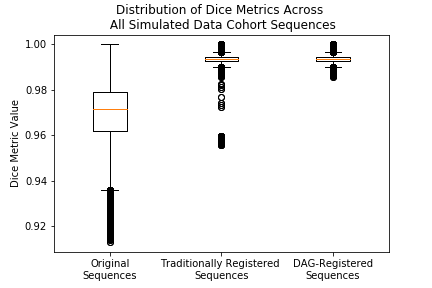
\includegraphics[height=0.3\textheight]{6/figures/spectr-dice-box.png}
\caption{Boxplots of the values of all Dice matrices for the original sequences, the traditionally registered sequences, and the DAG-registered sequences for the simulated data.}
\label{fig:spectr-dice-box}
\end{figure}

\begin{figure}
\centering
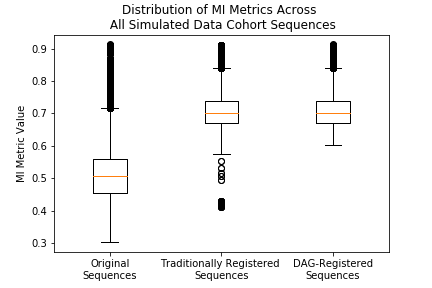
\includegraphics[height=0.3\textheight]{6/figures/spectr-mi-box.png}
\caption{Boxplots of the values of all MI matrices for the original sequences, the traditionally registered sequences, and the DAG-registered sequences for the simulated data.}
\label{fig:spectr-mi-box}
\end{figure}

The Dice and MI similarity matrices were calculated for each sequence. Box and whisker plots show the distributions of the metrics across the simulated data cohort for the Dice matrices and the mutual information matrices in Figures \ref{fig:spectr-dice-box} and \ref{fig:spectr-mi-box}, respectively.  


The Dice metric and MI matrices showed similar statistical differences, though these metrics have upper bound instead of a lower bound. The original sequences have statistically significantly different minimums, first quartiles, medians, and third quartiles from the registered sequences at $p < 0.005$ and similar maximum values. The p-values for these calculations can be seen in Table \ref{tab:spectr-dice-ttest} for the Dice matrices and Table \ref{tab:spectr-mi-ttest} for the MI matrices. 

The Kolmogorov-Smirnov test was used to compare the distributions for each metric. The tests showed that each pair of distributions for each metric type differed with a statistical significance of $p < 0.005$.

The analysis of sequence-level motion was performed using three metrics to measure the similarity of the volumes across each sequence. The matrices were compared to each other with respect to five descriptive statistics and with respect to the distribution of the entire set of similarity matrices for the original image sequences and each registration type. The distributions of the similarity metrics were found to be statistically significantly different, implying that each type of sequence contains different motion patterns.


\subsubsection{Volume Registration: Recovered Signal}

The registered images underwent independent component analysis (ICA) to identify signal components which contribute to the image as a whole. Traditionally, ICA is used to identify signal components correlated with a patient's motion so that they can be regressed out of the image sequence. Since the BOLD signal added to each simulated image is known, ICA can be used to determine how much BOLD signal is retained after volume registration.

ICA was applied to all registered sequences to identify the signal components. For each sequence, the components were compared to the DMN ROI. The components with the most significant correlation to the DMN ROI were categorized as the BOLD-related components. The average correlations between the BOLD-related components and the DMN ROI were 8122 for the traditionally registered sequences and 8040 for the DAG-registered sequences. The correlations for the two types of registered sequences were compared using both the Kolmogorov-Smirnov test and a two-sample t-test. Neither the test estimated a statistical significance between the correlation distributions for the registered sequences (KS p-value = 0.999; t-test p-value 0.807).

\begin{table}[]
\centering
\caption{The average rates and their confidence intervals for the classifications of component voxels as belonging to the DMN ROI for both types of registration.}
\label{tab:spectr-avg-rates}
\begin{tabular}{|c|c|c|}
\hline
\textbf{Average Value} & \textbf{Traditionally Registered} & \textbf{DAG-Registered} \\ \hline
TPR                    & 0.587 $\pm$ 0.0697                & 0.623 $\pm$ 0.0620      \\ \hline
FPR                    & 0.104 $\pm$ 0.00188               & 0.00996 $\pm$ 0.00180   \\ \hline
TNR                    & 0.990 $\pm$ 0.00188               & 0.990 $\pm$ 0.00180     \\ \hline
FNR                    & 0.413 $\pm$ 0.0697                & 0.377 $\pm$ 0.0620      \\ \hline
\end{tabular}
\end{table}

The accuracy of the BOLD-related components was determined by comparing the component image volumes to the DMN ROI on a voxel level. The absolute value of each BOLD-related component image volume was taken and thresholded at 10\% of the maximum absolute value. The thresholded BOLD-related component image volumes were compared to DMN ROI. With the DMN ROI used as ground truth, the counts of voxels, which were true positive, false positive, true negative, and false negative rates were calculated for each registration type. These values can be seen in Table \ref{tab:spectr-avg-rates}. The rates were compared for the traditionally registered and DAG-registered sequences. While none of the rates were statistically significant at even $ p < 0.05$, the rates were better for the DAG-registered sequences than for the traditionally registered sequences. 

\subsection{Preadolescent Cohort}

\subsubsection{Volume Registration: Power Thresholds}

\begin{figure}[]
	\centering
	\begin{subfigure}{0.4\textwidth}
		\centering
		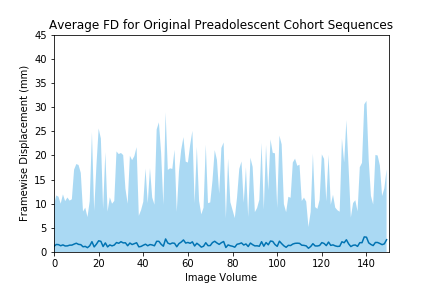
\includegraphics[width=1.0\textwidth]{6/figures/preads-bold-fd-150.png}
		\caption{FD of Original Sequences.}
	\end{subfigure}
	\hspace{0.05\textwidth}
	\begin{subfigure}{0.4\textwidth}
		\centering
		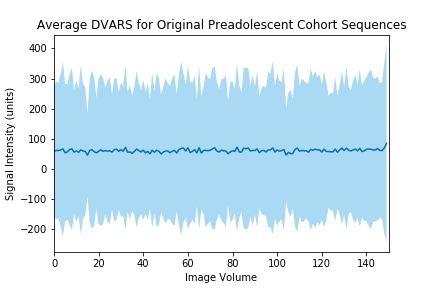
\includegraphics[width=1.0\textwidth]{6/figures/preads-bold-dvars-150.png}
		\caption{DVARS of Original Sequences.}
	\end{subfigure}
	
	\begin{subfigure}{0.4\textwidth}
		\centering
		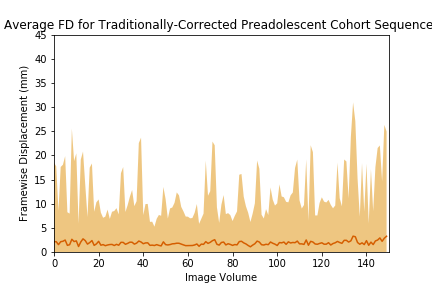
\includegraphics[width=1.0\textwidth]{6/figures/preads-trad-fd-150.png}
		\caption{FD of Traditionally Registered Sequences.}
	\end{subfigure}
	\hspace{0.05\textwidth}
	\begin{subfigure}{0.4\textwidth}
		\centering
		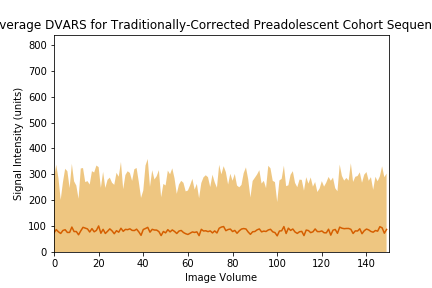
\includegraphics[width=1.0\textwidth]{6/figures/preads-trad-dvars-150.png}
		\caption{DVARS of Traditionally Registered Sequences.}
	\end{subfigure}
	
	\begin{subfigure}{0.4\textwidth}
		\centering
		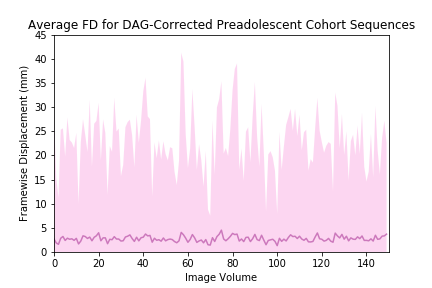
\includegraphics[width=1.0\textwidth]{6/figures/preads-dag-fd-150.png}
		\caption{FD of DAG-Registered Sequences.}
	\end{subfigure}
	\hspace{0.05\textwidth}
	\begin{subfigure}{0.4\textwidth}
		\centering
		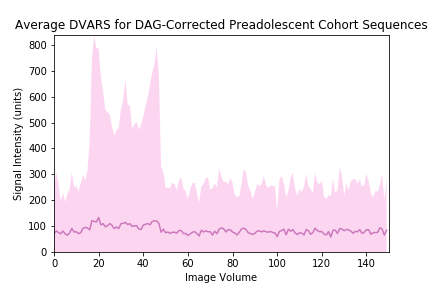
\includegraphics[width=1.0\textwidth]{6/figures/preads-dag-dvars-150.png}
		\caption{DVARS of DAG-Registered Sequences.}
	\end{subfigure}
\caption{The means and standard deviations of the FD and DVARS metrics for all preadolescent images before and after each type of registration.}
\label{fig:pread-power-dists}
\end{figure}

% First: FD and DVARs
The FD and DVARs were calculated for each original and registered preadolescent image sequences. The sequences varied in length from 150 volume to 450 volumes due to the differences in acquisition protocols at different sites. The number of image volumes used in this analysis was limited to the first 150 to avoid the challenges of comparing data with missing values.

The means and stand deviations of the FD and DVARS at each timepoint for each registration type can be seen in Figure \ref{fig:pread-power-dists}. The mean and standard deviation of the FD for the original sequences were 1.61 mm and 10.06 mm. The means of the FD increased to 1.83 mm for the traditionally registered sequences and 2.85 mm for the DAG-registered sequences. The standard deviation of the FD decreased to 7.74 mm for the traditionally registered sequences but increased to 15.4 mm for the DAG-registered sequences. The DVARS metrics followed a similar pattern: the mean of 60.5 units for the original sequences increased to 81.5 units and 92.5 units for the traditionally and DAG-registered sequences respectively while the standard deviation of the DVARS decreased from 197 units in the original sequences to 175 units in the traditionally registered sequences and increased to 284 units in the DAG-registered sequences.

\begin{table}[h]
\centering
\caption{The counts and percentages of image volumes across each type of sequence in the preadolescent cohort which meet the usability thresholds of FD $<$ 0.2 mm and DVARS $<$ 2.5\%.}
\label{tab:pread-power-thresh}
\begin{tabular}{|c|c|c|c|}
\hline
\textbf{Threshold} &
  \textbf{\begin{tabular}[c]{@{}c@{}}Original\\  Sequences\end{tabular}} &
  \textbf{\begin{tabular}[c]{@{}c@{}}Traditionally Registered \\ Sequences\end{tabular}} &
  \textbf{\begin{tabular}[c]{@{}c@{}}DAG-Registered \\ Sequences\end{tabular}} \\ \hline
FD     & 107879 (60.17\%) & 72104 (40.22\%) & 72114 (40.26\%) \\ \hline
DVARS  & 87169 (48.62\%) & 54056 (30.15\%) & 53756 (30.01\%) \\ \hline
Both   & 74107 (41.33\%) & 45006 (25.10\%) & 44682 (24.94\%) \\ \hline
\end{tabular}
\end{table}

The number of image volumes from each sequence type that met the FD and DVARS usability thresholds was calculated. The counts and percentages for each sequence type can be seen in Table \ref{tab:pread-power-thresh}. In the original image sequences, 60\% of image volumes met the FD threshold, 49\% of image volumes met the DVARS threshold, and 41\% of image volumes met both thresholds. After either registration, 40\% of image volumes met the FD threshold, 30\% of image volumes met the DVARS threshold, and about 25\% of image volumes met both thresholds.

The complete set of results can be seen in Table \ref{tab:pread-power-ttest}. The original image sequences were statistically significantly different from both types of registered image sequences with respect to the distributions of volumes meeting the FD threshold, the DVARS threshold, and both thresholds. The distributions for the registered image sequences were statistically similar for all three thresholds. 

\begin{table}[h]
\centering
\caption{The number of preadolescent subjects whose sequences of types $S_1$ and $S_2$ had statistically different FD distributions.}
\label{tab:pread-fd-kstest}
\begin{tabular}{|c|c|c|c|}
\hline
\textbf{\begin{tabular}[c]{@{}c@{}}\# Sequences \\ Type 1 ($S_1$)\end{tabular}} &
  \textbf{\begin{tabular}[c]{@{}c@{}}\# Sequences \\ Type 2 ($S_2$)\end{tabular}} &
  \textbf{\begin{tabular}[c]{@{}c@{}}\# Sequences \\ p $<$ 0.05\end{tabular}} &
  \textbf{\begin{tabular}[c]{@{}c@{}}\# Sequences \\ p $<$ 0.005\end{tabular}} \\ \hline
Original                                                            & \begin{tabular}[c]{@{}c@{}}Traditionally\\ Registered\end{tabular} & 331 & 326 \\ \hline
Original                                                            & \begin{tabular}[c]{@{}c@{}}DAG\\ Registered\end{tabular}           & 332 & 328 \\ \hline
\begin{tabular}[c]{@{}c@{}}Traditionally \\ Registered\end{tabular} & \begin{tabular}[c]{@{}c@{}}DAG\\ Registered\end{tabular}           & 19 &17 \\ \hline
\end{tabular}
\end{table}

\begin{table}[h]
\centering
\caption{The number of preadolescent subjects whose sequences of types $S_1$ and $S_2$ had statistically different DVARS distributions.}
\label{tab:pread-dvars-kstest}
\begin{tabular}{|c|c|c|c|}
\hline
\textbf{\begin{tabular}[c]{@{}c@{}}\# Sequences \\ Type 1 ($S_1$)\end{tabular}} &
  \textbf{\begin{tabular}[c]{@{}c@{}}\# Sequences \\ Type 2 ($S_2$)\end{tabular}} &
  \textbf{\begin{tabular}[c]{@{}c@{}}\# Sequences \\ p $<$ 0.05\end{tabular}} &
  \textbf{\begin{tabular}[c]{@{}c@{}}\# Sequences \\ p $<$ 0.005\end{tabular}} \\ \hline
Original                                                            & \begin{tabular}[c]{@{}c@{}}Traditionally\\ Registered\end{tabular} & 334 & 331 \\ \hline
Original                                                            & \begin{tabular}[c]{@{}c@{}}DAG\\ Registered\end{tabular}           & 334 & 333 \\ \hline
\begin{tabular}[c]{@{}c@{}}Traditionally \\ Registered\end{tabular} & \begin{tabular}[c]{@{}c@{}}DAG\\ Registered\end{tabular}           & 22  & 19  \\ \hline
\end{tabular}
\end{table}

The distributions of the FD and DVARS values were compared for each sequence type for each subject. For each subject, the distributions of each metric for the original and traditionally registered, the original and DAG-registered, and the traditional and DAG-registered sequences were compared using the Kolmogorov-Smirnov test. The results of these tests can be seen in Tables \ref{tab:pread-fd-kstest} and \ref{tab:pread-dvars-kstest}. Out of 545 images, approximately 330 had FD and DVARS distributions that were statistically significantly different between the original sequences and both types of registered sequences for $p < 0.005$. Between the two types of registered sequences, 19 and 17 had statistically significant differences in their FD distributions at $p < 0.05$ and $p < 0.005$, respectively. Similarly, 22 and 19 registered sequences had statistically significant differences in their DVARS distributions at $p < 0.05$ and $p < 0.005$. 

The comparison of the preadolescent sequences to the usability thresholds shows that either registration type increases the mean FD and DVARS metrics. The traditional registration method was shown to decrease the variance of the FD and DVARS metrics, but the DAG-based registration was shown to increase the variance of the FD and DVARS metrics. However, both registration types produced image sequences with similar numbers of image volumes meeting the FD threshold, the DVARS threshold, and both thresholds. The distributions of the FD and DVARS metrics were not statistically different for the two registration methods but were statistically significantly different between the original sequences and the registered sequences.


%The two-sided KS test measures the distance between the empirical distributions of two distributions. The null hypothesis of the two-sided KS test is that the empirical distributions being compared come from the same underlying distribution. As the KS test is nonparametric, the metrics for all image volumes can be used.

%By comparing the distributions for the original sequences to the distributions for the registered sequences, we aim to determine if the volume registration had a significant effect on the images themselves. The comparison of the distributions for the two types of registered images is intended to determine if there is a statistically significant difference between the FD and DVARS distributions of the registered images.


%An example of the three similarity matrices can be seen in Figure \ref{fig:sim-mat-sample}. The element $e_{i,j}$ represents the value of the given metric between the image volumes represented by row $i$ and column $j$. Each metric measures similarity according to slightly different definitions. In this figure, lighter values represent better metric values, while darker values indicate a lower similarity.
%
%It is important to note that the scales for these three metrics vary. The correlation ratio measures the distance between two items. Lower values for the correlation ratio means there is a smaller distance between the given pair of image volumes. The mutual information measures the shared information between two distributions of samples which may or may not be generated from the same underlying distribution. Higher mutual information values mean more shared information, and lower values mean less shared information. The Dice coefficient measures the overlap of two binary images. High Dice coefficients indicate a large amount of overlap, with a value of 1.0 indicating a perfect overlap.

%The correlation ratio matrix in Figure \ref{fig:sim-mat-sample} suggests that the patient remained relatively still for the first 300 volumes of the image, then moved for about 100 volumes, and remained still in a new position for the last 50 frames of the sequence. The colors representing the correlation ratios correspond to very low values, suggesting there is little patient motion overall.

%The Dice coefficient matrix has a similar pattern as the mutual information matrix, but leads to a different conclusion. The Dice coefficient was calculated on an Otsu thresholded version of each image volume. As the values of the Dice coefficients are consistently high, the patient likely did not move much. 
%
%The mutual information matrix shows that the shared information throughout the entire image sequence varies. Using the information from the correlation ratio matrix and the Dice coefficient matrix, it is possible that the variations in the mutual information matrix are due to changes in the rs-fMRI signal caused by BOLD signal changes, spin history effects of motion, and susceptibility effects of motion.

\subsubsection{Volume Registration: Sequence Duration Motion}

\begin{figure}[]
\centering
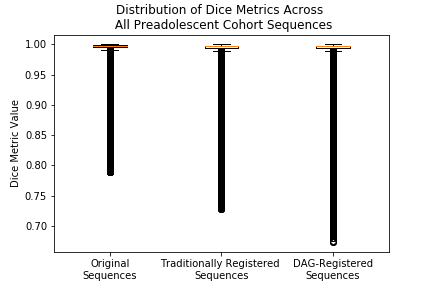
\includegraphics[height=0.3\textheight]{6/figures/preads-dice-box.png}
\caption{Boxplots of the values of all Dice matrices for the original sequences, the traditionally registered sequences, and the DAG-registered sequences for the preadolescent cohort.}
\label{fig:preads-dice-box}
\end{figure}

\begin{figure}[]
\centering
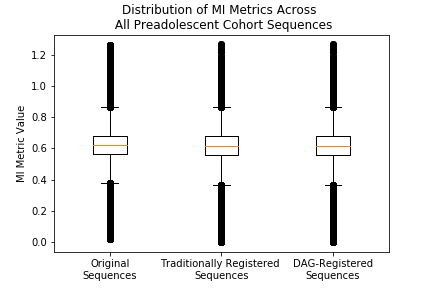
\includegraphics[height=0.3\textheight]{6/figures/preads-mi-box.png}
\caption{Boxplots of the values of all MI matrices for the original sequences, the traditionally registered sequences, and the DAG-registered sequences for the preadolescent cohort.}
\label{fig:preads-mi-box}
\end{figure}

For the preadolescent cohort, the Dice and MI matrices were calculated for the original, traditionally registered, and DAG-registered sequences. The distributions of the metric values for all matrices for each sequence can be seen in Figure \ref{fig:preads-dice-box} for the Dice matrices and in Figure \ref{fig:preads-mi-box} for the MI matrices. The minimums, first quantiles, medians, third quantiles, and maximums for each metric distribution were calculated. These descriptive statistics were compared to each other using the two-sample t-test for each sequence type. The only statistically significant difference in descriptive statistics for the Dice matrices was the difference between the third quartiles of the original sequences and both types of registered sequences at $p < 0.005$. There were no statistically significant differences between the descriptive statistics for the MI matrices, even at $p < 0.05$. The full results of these comparisons can be seen in Table \ref{appendix:results}.\ref{tab:preads-dice-ttest} for the Dice matrices and Table \ref{appendix:results}.\ref{tab:preads-mi-ttest} for the MI matrices.

\begin{table}[]
\centering
\caption{The number of preadolescent subjects whose sequences of types $S_1$ and $S_2$ had statistically different Dice distributions.}
\label{tab:preads-dice-kstest}
\begin{tabular}{|c|c|c|c|}
\hline
\textbf{\begin{tabular}[c]{@{}c@{}}\# Sequences \\ Type 1 ($S_1$)\end{tabular}} &
  \textbf{\begin{tabular}[c]{@{}c@{}}\# Sequences \\ Type 2 ($S_2$)\end{tabular}} &
  \textbf{\begin{tabular}[c]{@{}c@{}}\# Sequences \\ p $<$ 0.05\end{tabular}} &
  \textbf{\begin{tabular}[c]{@{}c@{}}\# Sequences \\ p $<$ 0.005\end{tabular}} \\ \hline
Original                                                            & \begin{tabular}[c]{@{}c@{}}Traditionally\\ Registered\end{tabular} & 188 & 185 \\ \hline
Original                                                            & \begin{tabular}[c]{@{}c@{}}DAG\\ Registered\end{tabular}           & 187 & 185 \\ \hline
\begin{tabular}[c]{@{}c@{}}Traditionally \\ Registered\end{tabular} & \begin{tabular}[c]{@{}c@{}}DAG\\ Registered\end{tabular}           & 83  & 75  \\ \hline
\end{tabular}
\end{table}

\begin{table}[]
\centering
\caption{The number of preadolescent subjects whose sequences of types $S_1$ and $S_2$ had statistically different MI distributions.}
\label{tab:preads-mi-kstest}
\begin{tabular}{|c|c|c|c|}
\hline
\textbf{\begin{tabular}[c]{@{}c@{}}\# Sequences \\ Type 1 ($S_1$)\end{tabular}} &
  \textbf{\begin{tabular}[c]{@{}c@{}}\# Sequences \\ Type 2 ($S_2$)\end{tabular}} &
  \textbf{\begin{tabular}[c]{@{}c@{}}\# Sequences \\ p $<$ 0.05\end{tabular}} &
  \textbf{\begin{tabular}[c]{@{}c@{}}\# Sequences \\ p $<$ 0.005\end{tabular}} \\ \hline
Original                                                            & \begin{tabular}[c]{@{}c@{}}Traditionally\\ Registered\end{tabular} & 189 & 187 \\ \hline
Original                                                            & \begin{tabular}[c]{@{}c@{}}DAG\\ Registered\end{tabular}           & 189 & 185 \\ \hline
\begin{tabular}[c]{@{}c@{}}Traditionally \\ Registered\end{tabular} & \begin{tabular}[c]{@{}c@{}}DAG\\ Registered\end{tabular}           & 84  & 69 \\ \hline
\end{tabular}
\end{table}

The distributions of the Dice and MI matrices across all three sequence types for each subject were compared using the Kolmogorov-Smirnov test. For the Dice metrics, the original sequences and the registered sequences had approximately 190 significantly different sequences at $p < 0.05$ and about 185 at $p < 0.005$. The traditionally registered and DAG-registered sequences had 84 sequences that were statistically different at $p < 0.05$ and 69 at $p < 0.005$. In the comparison of MI metrics for the original sequences and the traditionally registered sequences, 188 and 185 had statistically significant differences at $p < 0.05$ and $p < 0.005$. The original sequences and the DAG-registered sequences had similar differences at 187 and 185 significantly different sequences at $p < 0.05$ and $p < 0.005$. The traditionally registered and DAG-registered sequences had 83 and 75 statistically significantly different sequences at $p < 0.05$ and $p < 0.005$.

%Examining motion throughout the duration of the sequence showed that the two registration methods produced some image sequences with statistically different motion distributions 

Overall, the motion patterns embodied by the Dice and MI matrices were fairly similar for each metric across all three sequence types. A subset of images had statistically significant differences between the original sequences and the registered sequences for both the Dice and MI matrices, and a smaller subset had statistically significant differences between the two registration types. 

%-----------------------------------------------------------------
\subsection{Neonatal Cohort}

\subsubsection{Volume Registration: Power Thresholds}

\begin{figure}[]
	\centering
	\begin{subfigure}{0.4\textwidth}
		\centering
		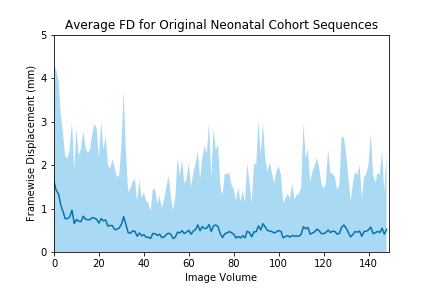
\includegraphics[width=1.0\textwidth]{6/figures/neonates-bold-fd-150.png}
		\caption{FD of Original Sequences.}
	\end{subfigure}
	\hspace{0.05\textwidth}
	\begin{subfigure}{0.4\textwidth}
		\centering
		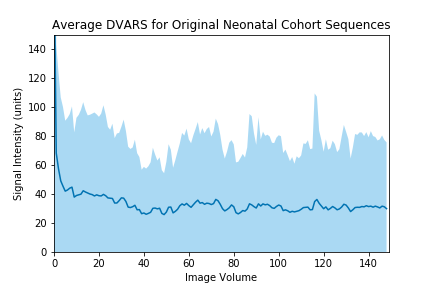
\includegraphics[width=1.0\textwidth]{6/figures/neonates-bold-dvars-150.png}
		\caption{DVARS of Original Sequences.}
	\end{subfigure}
	
	\begin{subfigure}{0.4\textwidth}
		\centering
		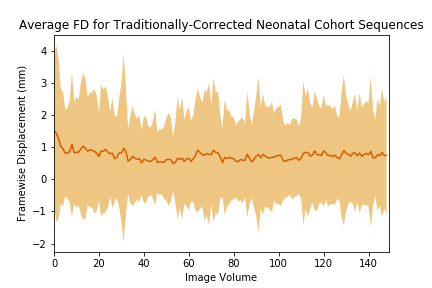
\includegraphics[width=1.0\textwidth]{6/figures/neonates-trad-fd-150.png}
		\caption{FD of Traditionally Registered Sequences.}
	\end{subfigure}
	\hspace{0.05\textwidth}
	\begin{subfigure}{0.4\textwidth}
		\centering
		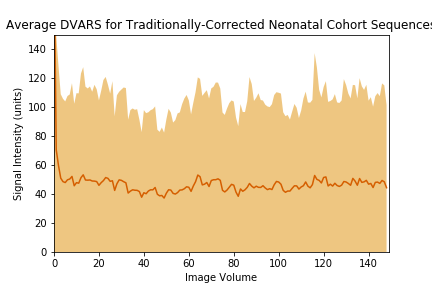
\includegraphics[width=1.0\textwidth]{6/figures/neonates-trad-dvars-150.png}
		\caption{DVARS of Traditionally Registered Sequences.}
	\end{subfigure}
	
	\begin{subfigure}{0.4\textwidth}
		\centering
		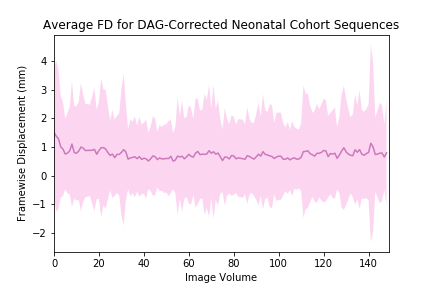
\includegraphics[width=1.0\textwidth]{6/figures/neonates-dag-fd-150.png}
		\caption{FD of DAG-Registered Sequences.}
	\end{subfigure}
	\hspace{0.05\textwidth}
	\begin{subfigure}{0.4\textwidth}
		\centering
		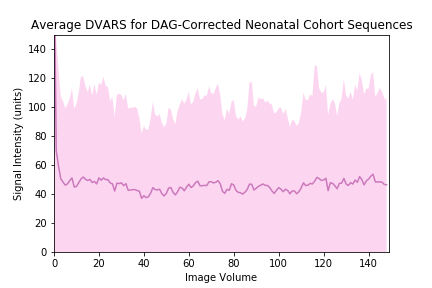
\includegraphics[width=1.0\textwidth]{6/figures/neonates-dag-dvars-150.png}
		\caption{DVARS of DAG-Registered Sequences.}
	\end{subfigure}
\caption{The means and standard deviations of the FD and DVARS metrics for all neonatal images before and after each type of registration.}
\label{fig:neonate-power-dists}
\end{figure}

\begin{table}[]
\centering
\caption{The counts and percentages of image volumes across each type of sequence in the neonatal cohort which meet the usability thresholds of FD $<$ 0.2 mm and DVARS $<$ 2.5\%.}
\label{tab:neonate-power-thresh}
\begin{tabular}{|c|c|c|c|}
\hline
\textbf{Threshold} &
  \textbf{\begin{tabular}[c]{@{}c@{}}Original\\  Sequences\end{tabular}} &
  \textbf{\begin{tabular}[c]{@{}c@{}}Traditionally Registered \\ Sequences\end{tabular}} &
  \textbf{\begin{tabular}[c]{@{}c@{}}DAG-Registered \\ Sequences\end{tabular}} \\ \hline
FD     & 16495 (69.59\%) & 14264 (60.18\%) & 14173 (59.79\%) \\ \hline
DVARS  & 16820 (70.96\%) & 13903 (58.65\%) & 13752 (58.02\%) \\ \hline
Both   & 15332 (64.68\%) & 12837 (54.16\%) & 12684 (53.51\%) \\ \hline
\end{tabular}
\end{table}

The FD and DVARs were calculated for the original and both types of registered sequences for the neonatal cohort. Each neonatal image was 150 volumes long. For each time point in the sequence, the mean and standard deviation of each metric for each image type was calculated. The means and standard deviations of these metric distributions can be seen in Figure \ref{fig:neonate-power-dists}. 

The original sequences had an average FD of 0.522 mm with a standard deviation of 0.787 mm. After registration, these values increased to an average of 0.740 mm and a standard deviation of 1.035 mm for the traditionally registered sequences and an average of 0.736 mm and a standard deviation of 1.036 mm for the DAG-registered sequences.

The DVARS metrics exhibited relationships between sequence types similar to the FD metrics. The average and standard deviation of the DVARS metrics for the original images were 34.1 units and 28.9 units. The traditionally registered sequences had a DVARS average and standard deviation of 47.1 units and 43.1 units, while the DAG-registered sequences had an average and standard deviation DVARS values of 46.8 units and 42.6 units. 

For each sequence, the number of image volumes which met the FD, DVARS, and joint FD and DVARS thresholds were calculated. The total number of image volumes across all sequences of a single type was 23704. The counts and percentages of neonatal image volumes meeting the thresholds can be seen in Table \ref{tab:neonate-power-thresh}. In the set of original image volumes, approximately 70\% of the volumes met the FD threshold and the DVARS threshold. This percentage decreased to about 65\% of the volumes when jointly considering the FD and DVARS thresholds. Both sets of registered image volumes had approximately 60\% of the image volumes meeting the FD threshold, 58\% of the image volumes meeting the DVARS threshold, and 54\% of the image volumes meeting both thresholds.

The statistical significance of the number of image volumes meeting each threshold was determined using two-sample t-tests. The three comparison pairs used were the original and traditionally registered sequences, the original and DAG-registered sequences, and the two types of registered sequences. The two types of registration did not have statistically significant differences in the number of image volumes meeting each threshold or the joint thresholds. The traditional registration had statistically significant differences from the number of image volumes in the original sequences in the number of image volumes meeting the FD threshold at $p < 0.05$ and the DVARS and joint thresholds at $p < 0.005$. The volume counts for the DAG-registered sequences significantly differed from the volume counts for the original sequences for the individual and joint thresholds at $p < 0.005$. A complete set of the precise p-values can be seen in Table \ref{appendix:results}.\ref{tab:neonate-power-ttest}.

\begin{table}[]
\centering
\caption{The number of neonatal subjects whose sequences of types $S_1$ and $S_2$ had statistically different FD distributions.}
\label{tab:neonate-fd-kstest}
\begin{tabular}{|c|c|c|c|}
\hline
\textbf{\begin{tabular}[c]{@{}c@{}}\# Sequences \\  Type 1 ($S_1$)\end{tabular}} &
  \textbf{\begin{tabular}[c]{@{}c@{}}\# Sequences \\ Type 2 ($S_2$)\end{tabular}} &
  \textbf{\begin{tabular}[c]{@{}c@{}}\# Sequences \\ p $<$ 0.05\end{tabular}} &
  \textbf{\begin{tabular}[c]{@{}c@{}}\# Sequences \\ p $<$ 0.005\end{tabular}} \\ \hline
Original                                                            & \begin{tabular}[c]{@{}c@{}}Traditionally\\ Registered\end{tabular} & 36	 & 32 \\ \hline
Original                                                            & \begin{tabular}[c]{@{}c@{}}DAG\\ Registered\end{tabular}           & 42 & 38 \\ \hline
\begin{tabular}[c]{@{}c@{}}Traditionally \\ Registered\end{tabular} & \begin{tabular}[c]{@{}c@{}}DAG\\ Registered\end{tabular}           & 13 & 5 \\ \hline
\end{tabular}
\end{table}

\begin{table}[]
\centering
\caption{The number of neonatal subjects whose sequences of types $S_1$ and $S_2$ had statistically different DVARS distributions.}
\label{tab:neonate-dvars-kstest}
\begin{tabular}{|c|c|c|c|}
\hline
\textbf{\begin{tabular}[c]{@{}c@{}}\# Sequences \\ Type 1($S_1$)\end{tabular}} &
  \textbf{\begin{tabular}[c]{@{}c@{}}\# Sequences \\ Type 2 ($S_2$)\end{tabular}} &
  \textbf{\begin{tabular}[c]{@{}c@{}}\# Sequences \\ p $<$ 0.05\end{tabular}} &
  \textbf{\begin{tabular}[c]{@{}c@{}}\# Sequences \\ p $<$ 0.005\end{tabular}} \\ \hline
Original                                                            & \begin{tabular}[c]{@{}c@{}}Traditionally\\ Registered\end{tabular} & 44 & 39 \\ \hline
Original                                                            & \begin{tabular}[c]{@{}c@{}}DAG\\ Registered\end{tabular}           & 45 & 44 \\ \hline
\begin{tabular}[c]{@{}c@{}}Traditionally \\ Registered\end{tabular} & \begin{tabular}[c]{@{}c@{}}DAG\\ Registered\end{tabular}           & 11  & 5  \\ \hline
\end{tabular}
\end{table}

For each image of all three sequence types, the distribution of the FD and DVARS metrics were compared using the Kolmogorov-Smirnov test. The number of images whose sequences of each type have different FD distributions can be seen in Table \ref{tab:neonate-fd-kstest}. The corresponding counts for the DVARS distributions can be seen in Table \ref{tab:neonate-dvars-kstest}. Following the pattern of the previous results presented in this section, there were more statistically significant differences between the original sequences and either type of registered sequence than between the two types of registered sequences. The registered images had consistent counts for both the FD and DVARS metrics: 13 sequences and 11 sequences had significantly different FD and DVARS distributions at $p < 0.05$, respectively, and both types had 5 sequences that were significantly different at $p < 0.005$. 

By comparing the FD and DVARS metrics of the original and registered sequences in several different ways, it has been established that images undergoing either type of registration differ from the original images. However, there was no statistically significant difference between the two types of registration with respect to the FD and DVARS metrics.

\subsubsection{Volume Registration: Sequence Duration Motion}

\begin{figure}
\centering
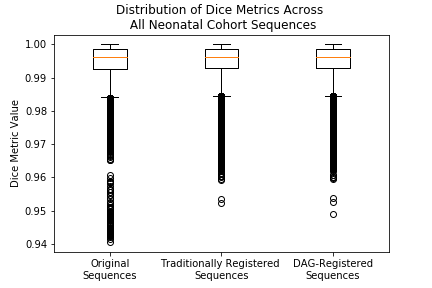
\includegraphics[width=0.5\textwidth]{6/figures/neonates-dice-box.png}
\caption{Boxplots of the values of all Dice matrices for the original sequences, the traditionally registered sequences, and the DAG-registered sequences for the neonatal cohort.}
\label{fig:neonates-dice-box}
\end{figure}

\begin{figure}
\centering
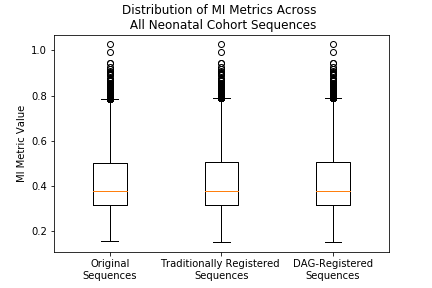
\includegraphics[width=0.5\textwidth]{6/figures/neonates-mi-box.png}
\caption{Boxplots of the values of all MI matrices for the original sequences, the traditionally registered sequences, and the DAG-registered sequences for the neonatal cohort.}
\label{fig:neonates-mi-box}
\end{figure}

Similarity matrices were computed to characterize patient motion throughout the duration of the image sequence. The value of each matrix at row $i$ column $j$ contains the similarity (either Dice or MI) between image volume $i$ and image volume $j$ in that sequence. The distributions of values for each metric type across the three sequence types can be seen in Figures \ref{fig:neonates-dice-box} and \ref{fig:neonates-mi-box}. The values of the minimum, first quartile, median, third quartile, and maximum were computed for each distribution. These values were compared using two-sample t-tests. No statistically significant difference was found between the original, traditionally registered, or DAG-registered sequences for either metric (complete values can be found in Tables \ref{appendix:results}.\ref{tab:neonates-dice-ttest} and \ref{appendix:results}.\ref{tab:neonates-mi-ttest}, respectively).

\begin{table}[]
\centering
\caption{The number of neonatal subjects whose sequences of types $S_1$ and $S_2$ had statistically different Dice distributions.}
\label{tab:neonates-dice-kstest}
\begin{tabular}{|c|c|c|c|}
\hline
\textbf{\begin{tabular}[c]{@{}c@{}}\# Sequences \\ Type 1 ($S_1$)\end{tabular}} &
  \textbf{\begin{tabular}[c]{@{}c@{}}\# Sequences \\ Type 2 ($S_2$)\end{tabular}} &
  \textbf{\begin{tabular}[c]{@{}c@{}}\# Sequences \\ p $<$ 0.05\end{tabular}} &
  \textbf{\begin{tabular}[c]{@{}c@{}}\# Sequences \\ p $<$ 0.005\end{tabular}} \\ \hline
Original                                                            & \begin{tabular}[c]{@{}c@{}}Traditionally\\ Registered\end{tabular} & 67 & 66 \\ \hline
Original                                                            & \begin{tabular}[c]{@{}c@{}}DAG\\ Registered\end{tabular}           & 71 & 69 \\ \hline
\begin{tabular}[c]{@{}c@{}}Traditionally \\ Registered\end{tabular} & \begin{tabular}[c]{@{}c@{}}DAG\\ Registered\end{tabular}           & 68 & 64  \\ \hline
\end{tabular}
\end{table}

\begin{table}[]
\centering
\caption{The number of neonatal subjects whose sequences of types $S_1$ and $S_2$ had statistically different MI distributions.}
\label{tab:neonates-mi-kstest}
\begin{tabular}{|c|c|c|c|}
\hline
\textbf{\begin{tabular}[c]{@{}c@{}}\# Sequences \\ Type 1 ($S_1$)\end{tabular}} &
  \textbf{\begin{tabular}[c]{@{}c@{}}\# Sequences \\ Type 2 ($S_2$)\end{tabular}} &
  \textbf{\begin{tabular}[c]{@{}c@{}}\# Sequences \\ p $<$ 0.05\end{tabular}} &
  \textbf{\begin{tabular}[c]{@{}c@{}}\# Sequences \\ p $<$ 0.005\end{tabular}} \\ \hline
Original                                                            & \begin{tabular}[c]{@{}c@{}}Traditionally\\ Registered\end{tabular} & 66 & 64 \\ \hline
Original                                                            & \begin{tabular}[c]{@{}c@{}}DAG\\ Registered\end{tabular}           & 71 & 69 \\ \hline
\begin{tabular}[c]{@{}c@{}}Traditionally \\ Registered\end{tabular} & \begin{tabular}[c]{@{}c@{}}DAG\\ Registered\end{tabular}           & 64 & 64  \\ \hline
\end{tabular}
\end{table}

The distributions of the metrics matrices were compared to each other using the Kolmogorov-Smirnov test for each pair of sequence types. The number of image sequences with statistically significantly different distributions can be seen in Table \ref{tab:neonates-dice-kstest} for the Dice metric and Table \ref{tab:neonates-mi-kstest} for the MI metric. For both metrics, about 70 image sequences differed at both $p < 0.05$ and $p < 0.005$ for all three pairs of sequence types.

The distributions of the similarity matrices were fairly similar across the whole neonatal cohort. However, the neonatal images have a greater number of statistically significantly different image sequences across all three sequence types than the simulated or the preadolescent images. There is also a higher statistical significance in the different images: at most, two image sequences had significant differences of $p < 0.05$ and greater than $p > 0.005$ for both metrics across all three sequence types.

\subsection{Fetal Cohort}

As discussed in the previous chapter, fetal patients experience different physical constraints than any post-natal population. There is no way to prevent a fetus from moving during a scan. As a result, not all scans used in this analysis could be obtained under ideal circumstances. The images are supposed to contain 100 image volumes, but this is not the case for every sequence. Out of the 123 brain images, one contained only 81 volumes, two contained only 75 volumes, and one contained only 33 volumes. Of the 101 placenta images, one contained only 95 volumes, one contained only 75 volumes, and one contained only 74 volumes. Additionally, not all sequences were able to undergo both types of registration successfully. 

The analyses for the fetal cohort are divided into two groups: analyses for the brain images and analyses for the placenta images. 

\subsubsection{Volume Registration: Power Thresholds, Fetal Brain}

\begin{figure}[]
	\centering
	\begin{subfigure}{0.4\textwidth}
		\centering
		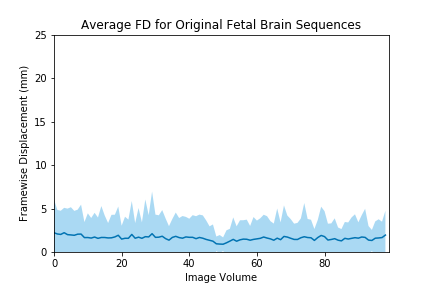
\includegraphics[width=1.0\textwidth]{6/figures/fetal-brain-bold-fd-150.png}
		\caption{FD of Original Sequences.}
	\end{subfigure}
	\hspace{0.05\textwidth}
	\begin{subfigure}{0.4\textwidth}
		\centering
		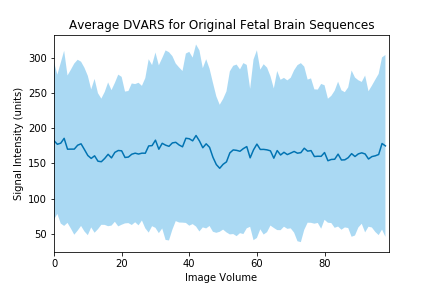
\includegraphics[width=1.0\textwidth]{6/figures/fetal-brain-bold-dvars-150.png}
		\caption{DVARS of Original Sequences.}
	\end{subfigure}
	
	\begin{subfigure}{0.4\textwidth}
		\centering
		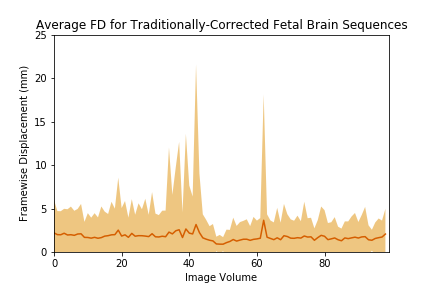
\includegraphics[width=1.0\textwidth]{6/figures/fetal-brain-trad-fd-150.png}
		\caption{FD of Traditionally Registered Sequences.}
	\end{subfigure}
	\hspace{0.05\textwidth}
	\begin{subfigure}{0.4\textwidth}
		\centering
		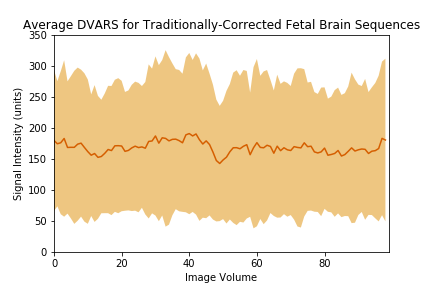
\includegraphics[width=1.0\textwidth]{6/figures/fetal-brain-trad-dvars-150.png}
		\caption{DVARS of Traditionally Registered Sequences.}
	\end{subfigure}
	
	\begin{subfigure}{0.4\textwidth}
		\centering
		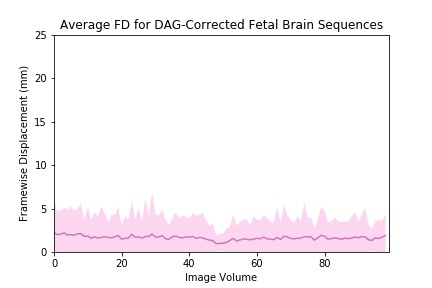
\includegraphics[width=1.0\textwidth]{6/figures/fetal-brain-dag-fd-150.png}
		\caption{FD of DAG-Registered Sequences.}
	\end{subfigure}
	\hspace{0.05\textwidth}
	\begin{subfigure}{0.4\textwidth}
		\centering
		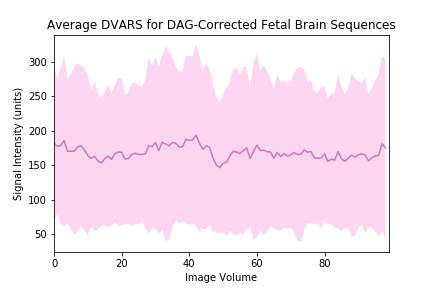
\includegraphics[width=1.0\textwidth]{6/figures/fetal-brain-dag-dvars-150.png}
		\caption{DVARS of DAG-Registered Sequences.}
	\end{subfigure}
\caption{The means and standard deviations of the FD and DVARS metrics for all fetal brain images before and after each type of registration.}
\label{fig:fetal-brain-power-dists}
\end{figure}

The FD and DVARS metrics were calculated for the fetal brain images. The averages and standard deviations of the FD and DVARS values across each point in time can be seen in Figure \ref{fig:fetal-brain-power-dists}. The FD for the original image sequences had an average of 1.61 mm and a standard deviation of 1.33 mm. These values increased for the traditionally registered image sequences to an average of 1.81 mm and a standard deviation of 1.90 mm. However, the average and standard deviation of the DAG-registered sequences were close to those of the original image sequences at an average of 1.64 mm and a standard deviation of 1.38 mm. The DVARS metrics for all three sequence types had similar distributions with averages of 167 units, 168 units, and 169 units and standard deviations of 74 units, 75 units, and 75 units, respectively.

\begin{table}[]
\centering
\caption{The count of and percentage of image volumes across each type of sequence in the fetal brain image data set which meet the usability thresholds of FD $<$ 0.2 mm and DVARS $<$ 2.5\%.}
\label{tab:fetal-brain-power-thresh}
\begin{tabular}{|c|c|c|c|}
\hline
\textbf{Threshold} &
  \textbf{\begin{tabular}[c]{@{}c@{}}Original\\  Sequences\end{tabular}} &
  \textbf{\begin{tabular}[c]{@{}c@{}}Traditionally Registered \\ Sequences\end{tabular}} &
  \textbf{\begin{tabular}[c]{@{}c@{}}DAG-Registered \\ Sequences\end{tabular}} \\ \hline
FD     & 575 (4.775\%)  & 581 (4.854\%) & 561 (4.659\%) \\ \hline
DVARS  & 7 (0.058\%)    & 84 (0.702\%)  & 7 (0.058\%) \\ \hline
Both   & 7 (0.058\%)    & 80 (0.668\%)  & 7 (0.058\%) \\ \hline
\end{tabular}
\end{table}

The FD and DVARS values for each image of each sequence type were compared to the usability thresholds. Table \ref{tab:fetal-brain-power-thresh} contains the number and percentages of image volumes that meet the FD threshold, the DVARS threshold, and the joint thresholds. Of the 12041 original image volumes, only 575 (4.78\%) met the FD threshold, and only 7 (0.058\%) met the DVARS and joint thresholds. For the traditionally registered image volumes, of which there were 11969, 581 (4.85\%) met the FD threshold, 84 (0.702\%) met the DVARS threshold, and 80 (0.668\%) met both thresholds. Again, the DAG-registered images closely followed the original images: of the 12041 image volumes, 561 (4.66\%) met the FD threshold, and 7 (0.058\%) met the DVARS and the joint thresholds. There was no statistically significant difference in the number of images meeting the thresholds between the three sequence types (complete set of p-values can be seen in Table \ref{appendix:results}.\ref{tab:fetal-brain-power-ttest}).

\begin{table}[]
\centering
\caption{The number of subjects whose sequences of types $S_1$ and $S_2$ had statistically different FD distributions according to the Kolmogorov-Smirnov test.}
\label{tab:fetal-brain-fd-kstest}
\begin{tabular}{|c|c|c|c|}
\hline
\textbf{\begin{tabular}[c]{@{}c@{}}\# Sequences \\ Type 1 ($S_1$)\end{tabular}} &
  \textbf{\begin{tabular}[c]{@{}c@{}}\# Sequences \\ Type 2 ($S_2$)\end{tabular}} &
  \textbf{\begin{tabular}[c]{@{}c@{}}\# Sequences \\ p $<$ 0.05\end{tabular}} &
  \textbf{\begin{tabular}[c]{@{}c@{}}\# Sequences \\ p $<$ 0.005\end{tabular}} \\ \hline
Original                                                            & \begin{tabular}[c]{@{}c@{}}Traditionally\\ Registered\end{tabular} & 14 & 9 \\ \hline
Original                                                            & \begin{tabular}[c]{@{}c@{}}DAG\\ Registered\end{tabular}           & 2  & 2 \\ \hline
\begin{tabular}[c]{@{}c@{}}Traditionally \\ Registered\end{tabular} & \begin{tabular}[c]{@{}c@{}}DAG\\ Registered\end{tabular}           & 13 & 9 \\ \hline
\end{tabular}
\end{table}

\begin{table}[]
\centering
\caption{The number of subjects whose sequences of types $S_1$ and $S_2$ had statistically different DVARS distributions according to the Kolmogorov-Smirnov test.}
\label{tab:fetal-brain-dvars-kstest}
\begin{tabular}{|c|c|c|c|}
\hline
\textbf{\begin{tabular}[c]{@{}c@{}}\# Sequences \\ Type 1 ($S_1$)\end{tabular}} &
  \textbf{\begin{tabular}[c]{@{}c@{}}\# Sequences \\ Type 2 ($S_2$)\end{tabular}} &
  \textbf{\begin{tabular}[c]{@{}c@{}}\# Sequences \\ p $<$ 0.05\end{tabular}} &
  \textbf{\begin{tabular}[c]{@{}c@{}}\# Sequences \\ p $<$ 0.005\end{tabular}} \\ \hline
Original                                                            & \begin{tabular}[c]{@{}c@{}}Traditionally\\ Registered\end{tabular} & 3 & 3 \\ \hline
Original                                                            & \begin{tabular}[c]{@{}c@{}}DAG\\ Registered\end{tabular}           & 2 & 1 \\ \hline
\begin{tabular}[c]{@{}c@{}}Traditionally \\ Registered\end{tabular} & \begin{tabular}[c]{@{}c@{}}DAG\\ Registered\end{tabular}           & 2  & 2  \\ \hline
\end{tabular}
\end{table}

On an image level, the distributions of each metric across each type of sequence for each image were compared. Tables \ref{tab:fetal-brain-fd-kstest} and \ref{tab:fetal-brain-dvars-kstest} contain the number of image sequences which were statistically different at $p < 0.05$ and $p < 0.005$ for the FD and DVARS metrics, respectively. These tables show that the original and the DAG-registered sequences were generally more similar than either the original or the DAG-registered sequences were to the traditionally registered sequences with respect to the FD. The distributions of the DVARS metrics were not identified as statistically different for any sequence type.

The FD and DVARS metrics suggest two concepts. First, the DAG-based registration produced image sequences that were more similar to the original sequences than the traditionally registered sequences were. Second, neither registration had a significant impact on the DVARS metrics.

\subsubsection{Volume Registration: Sequence Duration Motion, Fetal Brain}

\begin{figure}
\centering
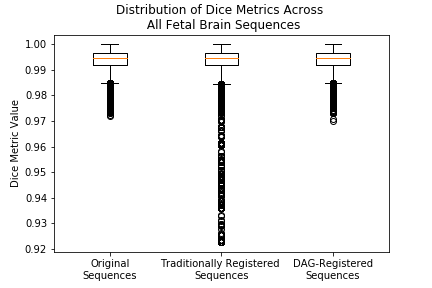
\includegraphics[width=0.5\textwidth]{6/figures/fetal-brain-dice-box.png}
\caption{Boxplots of the values of all Dice matrices for the original sequences, the traditionally registered sequences, and the DAG-registered sequences for the fetal-brain images.}
\label{fig:fetal-brain-dice-box}
\end{figure}

\begin{figure}
\centering
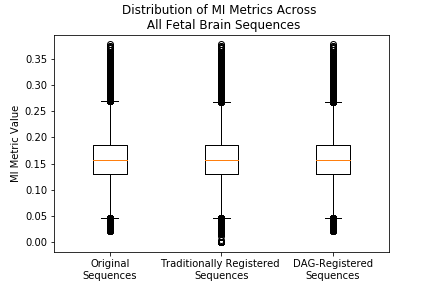
\includegraphics[width=0.5\textwidth]{6/figures/fetal-brain-mi-box.png}
\caption{Boxplots of the values of all MI matrices for the original sequences, the traditionally registered sequences, and the DAG-registered sequences for the fetal brain images.}
\label{fig:fetal-brain-mi-box}
\end{figure}

The changes in fetal brain position across the duration of the image sequences were measured using the similarity matrices. For each possible pair of image volumes $i$ and $j$, the value of the matrix at row $i$ column $j$ is the similarity of the two volumes. The two similarity metrics used were the Dice metric and the MI metric. The distributions of all values for every image of each sequence type can be seen in Figure \ref{fig:fetal-brain-dice-box} for the Dice metric and in Figure \ref{fig:fetal-brain-mi-box} for the MI metric.

The minimum, first quartile, median, third quartile, and maximum values for each distribution were calculated. These values were then compared using the two-sample t-test. No statistically significant difference was found between these values for any pair of sequence types for either the Dice matrices or the MI matrices. (For a complete list of p-values, see Tables \ref{appendix:results}.\ref{tab:fetal-brain-dice-ttest} and \ref{appendix:results}.\ref{tab:fetal-brain-mi-ttest}.

\begin{table}[]
\centering
\caption{The number of fetal brain images whose sequences of types $S_1$ and $S_2$ had statistically different Dice distributions.}
\label{tab:fetal-brain-dice-kstest}
\begin{tabular}{|c|c|c|c|}
\hline
\textbf{\begin{tabular}[c]{@{}c@{}}\# Sequences \\ Type 1 ($S_1$)\end{tabular}} &
  \textbf{\begin{tabular}[c]{@{}c@{}}\# Sequences \\ Type 2 ($S_2$)\end{tabular}} &
  \textbf{\begin{tabular}[c]{@{}c@{}}\# Sequences \\ p $<$ 0.05\end{tabular}} &
  \textbf{\begin{tabular}[c]{@{}c@{}}\# Sequences \\ p $<$ 0.005\end{tabular}} \\ \hline
Original                                                            & \begin{tabular}[c]{@{}c@{}}Traditionally\\ Registered\end{tabular} & 11 & 9 \\ \hline
Original                                                            & \begin{tabular}[c]{@{}c@{}}DAG\\ Registered\end{tabular}           & 7 & 7 \\ \hline
\begin{tabular}[c]{@{}c@{}}Traditionally \\ Registered\end{tabular} & \begin{tabular}[c]{@{}c@{}}DAG\\ Registered\end{tabular}           & 10  & 8  \\ \hline
\end{tabular}
\end{table}

\begin{table}[]
\centering
\caption{The number of fetal brain images whose sequences of types $S_1$ and $S_2$ had statistically different MI distributions.}
\label{tab:fetal-brain-mi-kstest}
\begin{tabular}{|c|c|c|c|}
\hline
\textbf{\begin{tabular}[c]{@{}c@{}}\# Sequences \\ Type 1 ($S_1$)\end{tabular}} &
  \textbf{\begin{tabular}[c]{@{}c@{}}\# Sequences \\ Type 2 ($S_2$)\end{tabular}} &
  \textbf{\begin{tabular}[c]{@{}c@{}}\# Sequences \\ p $<$ 0.05\end{tabular}} &
  \textbf{\begin{tabular}[c]{@{}c@{}}\# Sequences \\ p $<$ 0.005\end{tabular}} \\ \hline
Original                                                            & \begin{tabular}[c]{@{}c@{}}Traditionally\\ Registered\end{tabular} & 13 & 10 \\ \hline
Original                                                            & \begin{tabular}[c]{@{}c@{}}DAG\\ Registered\end{tabular}           & 12 & 9 \\ \hline
\begin{tabular}[c]{@{}c@{}}Traditionally \\ Registered\end{tabular} & \begin{tabular}[c]{@{}c@{}}DAG\\ Registered\end{tabular}           & 14 & 9  \\ \hline
\end{tabular}
\end{table}

The distributions of values in each matrix for each subject were compared to each other using the Kolmogorov-Smirnov test. The number of sequence comparisons that were statistically significant for the Dice metrics can be seen in Table \ref{tab:fetal-brain-dice-kstest}. Very few sequences had significantly different Dice distributions: between the three sequence types, only 7 to 11 sequences were statistically different at $p < 0.05$, and only 7 to 9 sequences were different at $p < 0.005$. The number of sequence comparisons that were statistically significant for the MI metrics can be seen in Table \ref{tab:fetal-brain-mi-kstest}. Similar to the Dice metrics, only 12 to 14 sequences were different at $p < 0.05$ and only 9 to 10 sequences were different at $p < 0.005$.

Overall, the distributions of the similarity metric matrices between the three sequences types were not statistically different.

\subsubsection{Volume Registration: Power Thresholds, Placenta}

\begin{figure}[]
	\centering
	\begin{subfigure}{0.4\textwidth}
		\centering
		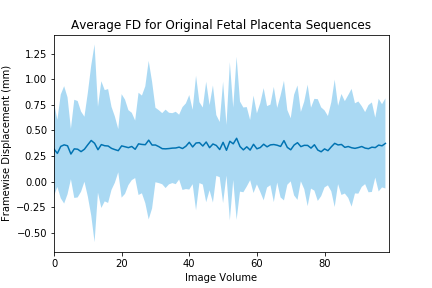
\includegraphics[width=1.0\textwidth]{6/figures/fetal-placenta-bold-fd-150.png}
		\caption{FD of Original Sequences.}
	\end{subfigure}
	\hspace{0.05\textwidth}
	\begin{subfigure}{0.4\textwidth}
		\centering
		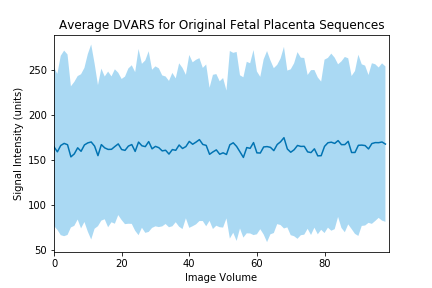
\includegraphics[width=1.0\textwidth]{6/figures/fetal-placenta-bold-dvars-150.png}
		\caption{DVARS of Original Sequences.}
	\end{subfigure}
	
	\begin{subfigure}{0.4\textwidth}
		\centering
		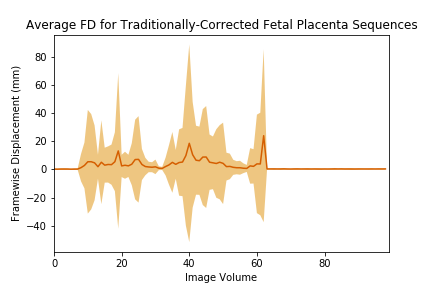
\includegraphics[width=1.0\textwidth]{6/figures/fetal-placenta-trad-fd-150.png}
		\caption{FD of Traditionally Registered Sequences.}
	\end{subfigure}
	\hspace{0.05\textwidth}
	\begin{subfigure}{0.4\textwidth}
		\centering
		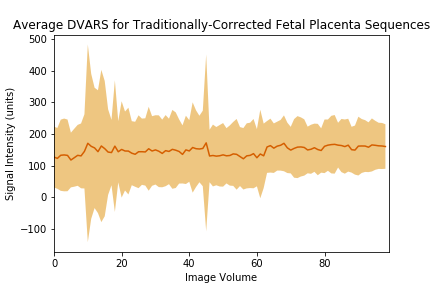
\includegraphics[width=1.0\textwidth]{6/figures/fetal-placenta-trad-dvars-150.png}
		\caption{DVARS of Traditionally Registered Sequences.}
	\end{subfigure}
	
	\begin{subfigure}{0.4\textwidth}
		\centering
		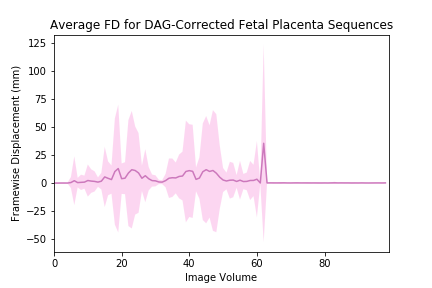
\includegraphics[width=1.0\textwidth]{6/figures/fetal-placenta-dag-fd-150.png}
		\caption{FD of DAG-Registered Sequences.}
	\end{subfigure}
	\hspace{0.05\textwidth}
	\begin{subfigure}{0.4\textwidth}
		\centering
		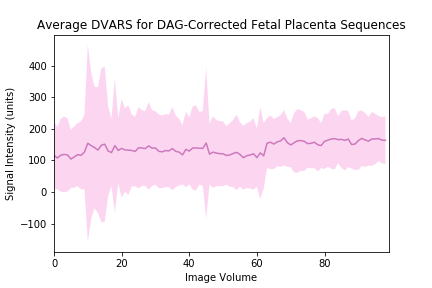
\includegraphics[width=1.0\textwidth]{6/figures/fetal-placenta-dag-dvars-150.png}
		\caption{DVARS of DAG-Registered Sequences.}
	\end{subfigure}
\caption{The means and standard deviations of the FD and DVARS metrics for all placenta images before and after each type of registration.}
\label{fig:fetal-placenta-power-dists}
\end{figure}

The FD and DVARS values for the placental images were calculated. The averages and standard deviations for the metric values at each time point in the sequence can be seen in Figure \ref{fig:fetal-placenta-power-dists}. The original sequences had an average FD of 0.341 mm with a standard deviation of 0.382 mm and an average DVARS of 163 units with a standard deviation of 73.8 units. The FD values increased after registration: the traditionally registered images had an average FD of 4.17 mm with a standard deviation of 8.67 mm, and the DAG-registered images had an average FD of 5.12 mm with a standard deviation of 9.14 mm. Registration had a different effect on the DVARS values. The average DVARS values decreased to 140 units for the traditionally registered sequences and to 127 units for the DAG-registered sequences. The standard deviation of the DVARS values increased, though, to 85.7 units for the traditionally registered images and to 91.9 units for the DAG-registered images. 

\begin{table}[]
\centering
\caption{The count of and percentage of image volumes across each type of sequence in the fetal placenta image data set which meet the usability thresholds of FD $<$ 0.2 mm and DVARS $<$ 2.5\%.}
\label{tab:fetal-placenta-power-thresh}
\begin{tabular}{|c|c|c|c|}
\hline
\textbf{Threshold} &
  \textbf{\begin{tabular}[c]{@{}c@{}}Original\\  Sequences\end{tabular}} &
  \textbf{\begin{tabular}[c]{@{}c@{}}Traditionally Registered \\ Sequences\end{tabular}} &
  \textbf{\begin{tabular}[c]{@{}c@{}}DAG-Registered \\ Sequences\end{tabular}} \\ \hline
FD     & 10017 (43.646\%) & 4113 (44.245\%)  & 4005 (45.020\%)   \\ \hline
DVARS  & 17 (0.170\%)    & 1056 (11.36\%)  & 1624 (18.255\%)  \\ \hline
Both   & 17 (0.170\%)   & 599 (6.444\%)    & 996 (11.196\%)   \\ \hline
\end{tabular}
\end{table}

The FD and DVARS values were compared to the usability thresholds. Table \ref{tab:fetal-placenta-power-thresh} contains the number and percentages of image volumes from all placenta sequence that meet the FD, the DVARS, and the joint thresholds. The total number of image volumes across the original sequences was 10017, the number of traditionally registered images was 9296, and the number of DAG-registered images was 8896. 

Of the original image volumes, 10017 (43.6\%) met the FD threshold. Only 17 (0.170\%) original image volumes met the DVARS threshold and the FD and DVARS thresholds. Both registration techniques reduced the number of image volumes, which met the FD thresholds to 4113 (44.245\%) volumes for the traditionally registered sequences and 4005 (45.1\%) for the DAG-registered sequences. The registration techniques increased the number of image volumes which met the DVARS threshold and the FD and DVARS thresholds. After traditional registration, 1056 (11.4\%) volumes met the DVARS threshold and 599 (6.44\%) met both thresholds. After DAG-based registration, 1624 (18.3\%) volumes met the DVARS threshold and 996 (11.2\%) volumes met both thresholds. Two-sample t-tests, the results of which can be found in Table \ref{appendix:results}.\ref{tab:fetal-placenta-power-ttest}, showed that the differences in the number of image volumes meeting the DVARS thresholds and the joint thresholds between the original sequences and the registered sequences are statistically significant at $p < 0.005$.

\begin{table}[]
\centering
\caption{The number of placental images whose sequences of types $S_1$ and $S_2$ had statistically different FD distributions according to the Kolmogorov-Smirnov test.}
\label{tab:fetal-placenta-fd-kstest}
\begin{tabular}{|c|c|c|c|}
\hline
\textbf{\begin{tabular}[c]{@{}c@{}}\# Sequences \\ Type 1 ($S_1$)\end{tabular}} &
  \textbf{\begin{tabular}[c]{@{}c@{}}\# Sequences \\ Type 2 ($S_2$)\end{tabular}} &
  \textbf{\begin{tabular}[c]{@{}c@{}}\# Sequences \\ p $<$ 0.05\end{tabular}} &
  \textbf{\begin{tabular}[c]{@{}c@{}}\# Sequences \\ p $<$ 0.005\end{tabular}} \\ \hline
Original                                                            & \begin{tabular}[c]{@{}c@{}}Traditionally\\ Registered\end{tabular} & 21 & 21 \\ \hline
Original                                                            & \begin{tabular}[c]{@{}c@{}}DAG\\ Registered\end{tabular}           & 32 & 30 \\ \hline
\begin{tabular}[c]{@{}c@{}}Traditionally \\ Registered\end{tabular} & \begin{tabular}[c]{@{}c@{}}DAG\\ Registered\end{tabular}           & 31 & 20 \\ \hline
\end{tabular}
\end{table}

\begin{table}[]
\centering
\caption{The number of placental images whose sequences of types $S_1$ and $S_2$ had statistically different DVARS distributions according to the Kolmogorov-Smirnov test.}
\label{tab:fetal-placenta-dvars-kstest}
\begin{tabular}{|c|c|c|c|}
\hline
\textbf{\begin{tabular}[c]{@{}c@{}}\# Sequences \\ Type 1 ($S_1$)\end{tabular}} &
  \textbf{\begin{tabular}[c]{@{}c@{}}\# Sequences \\ Type 2 ($S_2$)\end{tabular}} &
  \textbf{\begin{tabular}[c]{@{}c@{}}\# Sequences \\ p $<$ 0.05\end{tabular}} &
  \textbf{\begin{tabular}[c]{@{}c@{}}\# Sequences \\ p $<$ 0.005\end{tabular}} \\ \hline
Original                                                            & \begin{tabular}[c]{@{}c@{}}Traditionally\\ Registered\end{tabular} & 20 & 20 \\ \hline
Original                                                            & \begin{tabular}[c]{@{}c@{}}DAG\\ Registered\end{tabular}           & 29 & 29 \\ \hline
\begin{tabular}[c]{@{}c@{}}Traditionally \\ Registered\end{tabular} & \begin{tabular}[c]{@{}c@{}}DAG\\ Registered\end{tabular}           & 19 & 19  \\ \hline
\end{tabular}
\end{table}

For each placenta image, the distribution of the FD and DVARS metrics for each sequence type were compared using the Kolmogorov-Smirnov test. The results of these tests can be seen in Table \ref{tab:fetal-placenta-fd-kstest} and Table \ref{tab:fetal-placenta-dvars-kstest}.

The number of sequences which had statistically different FD distributions across all three sequence types can be seen in Table \ref{tab:fetal-placenta-fd-kstest}. The original and traditionally registered sequences had 21 sequences with significantly different FD at both $p < 0.05$ and $p < 0.005$. The original and DAG-registered sequences had 32 and 30 sequences with statistically different FD at $p < 0.05$ and $p < 0.005$, respectively. The two types of registration have 31 and 20 sequences with statistically different FD at $p < 0.05$ and $p < 0.005$. To summarize, approximately 20\% to 30\% of the images had statistically significantly different FD distributions depending on the sequence type.

With respect to the DVARS distributions, the traditionally registered sequences were more similar to the original sequences or the DAG-registered sequences. There were about 20 sequences that had different DVARS distributions between the traditionally registered sequences and the original and DAG-registered sequences at $p < 0.005$. The original and DAG-registered sequences were slightly less similar with 29 sequences between them which had different DVARS distributions at $p < 0.005$.

The FD distributions were not significantly different for the original and registered placenta sequences. However, the placenta images are the first images in our analyses which demonstrate an improvement in DVARS metrics after registration.

\subsubsection{Volume Registration: Sequence Duration Motion, Placenta}

\begin{figure}
\centering
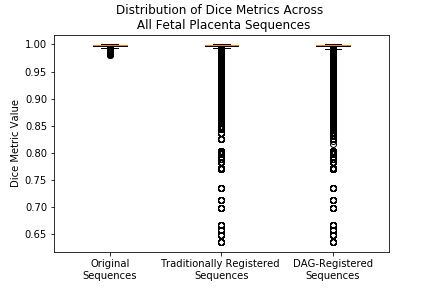
\includegraphics[width=0.5\textwidth]{6/figures/fetal-placenta-dice-box.png}
\caption{Boxplots of the values of all Dice matrices for the original sequences, the traditionally registered sequences, and the DAG-registered sequences for the placenta images.}
\label{fig:fetal-placenta-dice-box}
\end{figure}

\begin{table}[]
\centering
\caption{Results of t-tests comparing the descriptive statistics of the Dice matrices for the fetal placenta data.}
\label{tab:fetal-placenta-dice-ttest}
\begin{tabular}{|c|c|c|c|}
\hline
\textbf{Sequence Type 1 ($S_1$)} &
  \textbf{Original} &
  \textbf{Original} &
  \textbf{\begin{tabular}[c]{@{}c@{}}Traditionally \\ Registered\end{tabular}} \\ \hline
\textbf{Sequence Type 2 ($S_2$)} &
  \textbf{\begin{tabular}[c]{@{}c@{}}Traditionally\\ Registered\end{tabular}} &
  \textbf{\begin{tabular}[c]{@{}c@{}}DAG\\ Registered\end{tabular}} &
  \textbf{\begin{tabular}[c]{@{}c@{}}DAG\\ Registered\end{tabular}} \\ \hline
\begin{tabular}[c]{@{}c@{}}P($S_1$ and $S_2$ \\ have same minimums)\end{tabular} &
  6.39 E -5 &
  3.43 E -7 &
  0.257 \\ \hline
\begin{tabular}[c]{@{}c@{}}P($S_1$ and $S_2$ \\ have same 1st quartile)\end{tabular} &
  6.54 E -5 &
  2.35 E -6 &
  0.257 \\ \hline
\begin{tabular}[c]{@{}c@{}}P($S_1$ and $S_2$ \\ have same medians)\end{tabular} &
  0.000310 &
  9.46 E -5 &
  0.816 \\ \hline
\begin{tabular}[c]{@{}c@{}}P($S_1$ and $S_2$ \\ have same 3rd quartiles)\end{tabular} &
  0.096 &
  0.104 &
  0.902 \\ \hline
\begin{tabular}[c]{@{}c@{}}P($S_1$ and $S_2$ \\ have same maximums)\end{tabular} &
  1.0 &
  1.0 &
  1.0 \\ \hline
\end{tabular}
\end{table}

\begin{figure}
\centering
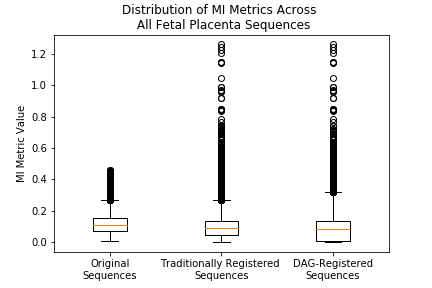
\includegraphics[width=0.5\textwidth]{6/figures/fetal-placenta-mi-box.png}
\caption{Boxplots of the values of all MI matrices for the original sequences, the traditionally registered sequences, and the DAG-registered sequences for the placenta images.}
\label{fig:fetal-placenta-mi-box}
\end{figure}

\begin{table}[]
\centering
\caption{Results of t-tests comparing the descriptive statistics of the MI matrices for the fetal placenta data.}
\label{tab:fetal-placenta-mi-ttest}
\begin{tabular}{|c|c|c|c|}
\hline
\textbf{Sequence Type 1 ($S_1$)} &
  \textbf{Original} &
  \textbf{Original} &
  \textbf{\begin{tabular}[c]{@{}c@{}}Traditionally \\ Registered\end{tabular}} \\ \hline
\textbf{Sequence Type 2 ($S_2$)} &
  \textbf{\begin{tabular}[c]{@{}c@{}}Traditionally\\ Registered\end{tabular}} &
  \textbf{\begin{tabular}[c]{@{}c@{}}DAG\\ Registered\end{tabular}} &
  \textbf{\begin{tabular}[c]{@{}c@{}}DAG\\ Registered\end{tabular}} \\ \hline
\begin{tabular}[c]{@{}c@{}}P($S_1$ and $S_2$ \\ have same minimums)\end{tabular} &
  0.00980 &
  0.00168 &
  0.536 \\ \hline
\begin{tabular}[c]{@{}c@{}}P($S_1$ and $S_2$ \\ have same 1st quartile)\end{tabular} &
  0.00742 &
  0.00132 &
  0.548 \\ \hline
\begin{tabular}[c]{@{}c@{}}P($S_1$ and $S_2$ \\ have same medians)\end{tabular} &
  0.00713 &
  0.00116 &
  0.535 \\ \hline
\begin{tabular}[c]{@{}c@{}}P($S_1$ and $S_2$ \\ have same 3rd quartiles)\end{tabular} &
  0.00807 &
  0.00118 &
  0.506 \\ \hline
\begin{tabular}[c]{@{}c@{}}P($S_1$ and $S_2$ \\ have same maximums)\end{tabular} &
  0.00145 &
  8.28 E -6 &
  0.212 \\ \hline
\end{tabular}
\end{table}

The image volumes across each sequence were compared by calculating the similarity between volume $i$ to volume $j$ and storing the results in row $i$ column $j$ of a 2D matrix for that sequence's similarity metric. The similarity metrics used for these comparisons were the Dice metric and the MI metric. The distributions of the values of each metric for each sequence type can be seen in Figure \ref{fig:fetal-placenta-dice-box} and Figure \ref{fig:fetal-placenta-mi-box} for the Dice and MI matrices, respectively. These distributions were compared by performing two-sample t-tests on the minimum, first quartile, median, third quartile, and maximum values for each sequence type. 

Table \ref{tab:fetal-placenta-dice-ttest} shows the results of the t-tests comparing the descriptive statistics for the Dice matrices. The minimum values, first quartiles, and medians were statistically different at $p < 0.005$ for the original and traditionally registered sequences as well as for the original and DAG-registered sequences. There was no significant difference between the third quartiles and the maximum values between the original and registered sequences. Additionally, there was no significant difference between the descriptive statistics for the traditionally and DAG-registered sequences.

The results of the t-tests comparing the descriptive statistics for the MI matrices can be seen in Table \ref{tab:fetal-placenta-mi-ttest}. The differences in all five statistics between the original sequences and the traditionally registered sequences were significant at $p < 0.05$. The differences between the original and DAG-registered sequences for all five statistics were significant at $p < 0.005$. There was no significant difference in the descriptive statistics for the MI matrix distributions between the traditionally registered and DAG-registered sequences.

\begin{table}[]
\centering
\caption{The number of subjects whose placenta sequences of types $S_1$ and $S_2$ had statistically different Dice distributions.}
\label{tab:fetal-placenta-dice-kstest}
\begin{tabular}{|c|c|c|c|}
\hline
\textbf{\begin{tabular}[c]{@{}c@{}}\# Sequences \\ Type 1 ($S_1$)\end{tabular}} &
  \textbf{\begin{tabular}[c]{@{}c@{}}\# Sequences \\ Type 2 ($S_2$)\end{tabular}} &
  \textbf{\begin{tabular}[c]{@{}c@{}}\# Sequences \\ p $<$ 0.05\end{tabular}} &
  \textbf{\begin{tabular}[c]{@{}c@{}}\# Sequences \\ p $<$ 0.005\end{tabular}} \\ \hline
Original                                                            & \begin{tabular}[c]{@{}c@{}}Traditionally\\ Registered\end{tabular} & 22 & 22 \\ \hline
Original                                                            & \begin{tabular}[c]{@{}c@{}}DAG\\ Registered\end{tabular}           & 39 & 39 \\ \hline
\begin{tabular}[c]{@{}c@{}}Traditionally \\ Registered\end{tabular} & \begin{tabular}[c]{@{}c@{}}DAG\\ Registered\end{tabular}           & 30 & 30  \\ \hline
\end{tabular}
\end{table}

\begin{table}[]
\centering
\caption{The number of subjects whose placenta sequences of types $S_1$ and $S_2$ had statistically different MI distributions.}
\label{tab:fetal-placenta-mi-kstest}
\begin{tabular}{|c|c|c|c|}
\hline
\textbf{\begin{tabular}[c]{@{}c@{}}\# Sequences \\ Type 1 ($S_1$)\end{tabular}} &
  \textbf{\begin{tabular}[c]{@{}c@{}}\# Sequences \\ Type 2 ($S_2$)\end{tabular}} &
  \textbf{\begin{tabular}[c]{@{}c@{}}\# Sequences \\ p $<$ 0.05\end{tabular}} &
  \textbf{\begin{tabular}[c]{@{}c@{}}\# Sequences \\ p $<$ 0.005\end{tabular}} \\ \hline
Original                                                            & \begin{tabular}[c]{@{}c@{}}Traditionally\\ Registered\end{tabular} & 22 & 22 \\ \hline
Original                                                            & \begin{tabular}[c]{@{}c@{}}DAG\\ Registered\end{tabular}           & 39 & 39 \\ \hline
\begin{tabular}[c]{@{}c@{}}Traditionally \\ Registered\end{tabular} & \begin{tabular}[c]{@{}c@{}}DAG\\ Registered\end{tabular}           & 38 & 38  \\ \hline
\end{tabular}
\end{table}


The distributions of the matrix values were compared on a subject level. These comparisons consisted of using the Kolmogorov-Smirnov test to determine if the distributions of the matrix values for two sequence types for the same subject were statistically different. The results of these comparisons can be seen in Table \ref{tab:fetal-placenta-dice-kstest} for the Dice matrices and in Table \ref{tab:fetal-placenta-mi-kstest} for the MI matrices. For both the Dice and MI comparisons, there were 22 sequences between the original and traditionally registered sequences which were statistically different at $p < 0.005$. The Dice and MI comparisons also both had 39 statistically different sequences between the original and DAG-registered sequences at $p < 0.005$. The traditionally and DAG-registered sequences had 38 statistically different sequences for the Dice comparison and 30 statistically different sequences for the MI comparison.

The similarity matrices for the placenta images suggest that the two registration types both produce sequences that have similarity distributions that are different from those of the original sequences. The two registration types differ in the metric distributions for some images, but over a population these differences are not significant.

\section{Characterizing Motion Across Clinical Groups}

Between the preadolescent, neonatal, and fetal brain images, we have a fairly large set of images. The images come from a population that is diverse and well represented in two areas: disease status and general patient age group. In this section, we compare groups of images identified using only the metrics discussed earlier in this chapter to these two groups of interest. 

As the goal of this analysis is to characterize patient motion, only the metrics for the original, unregistered sequences were used. These metrics exist in high dimensional spaces. In the high dimensional space, outlier vectors greater than three standard deviations from the mean vector were removed. The remaining feature vectors were clustered in the high dimensional spaces and then projected into 2D spaces for visualization purposes.

\subsection{CHD and Control}

\begin{figure}
\centering
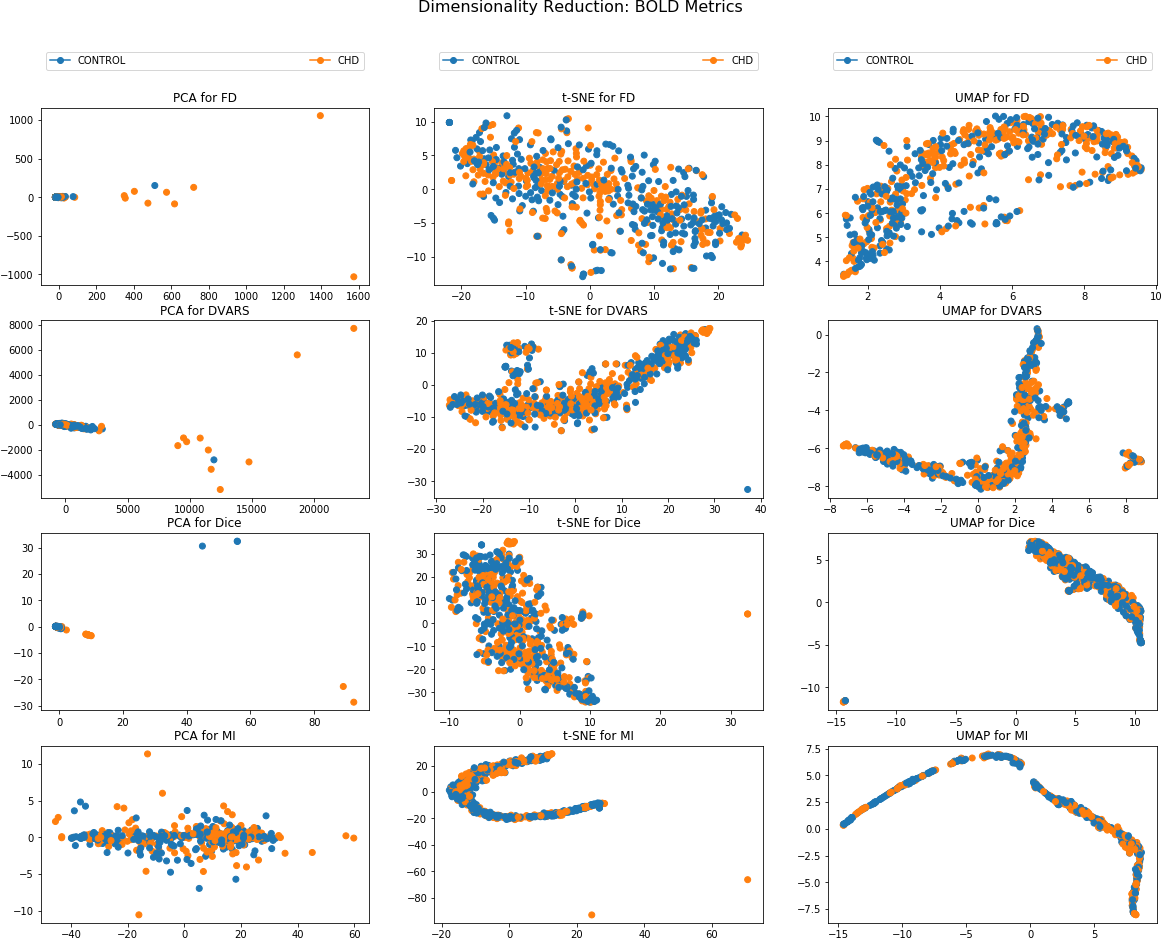
\includegraphics[width=1.0\textwidth]{6/figures/bold-2d-all-cohort.png}
\caption{The data for the four metrics used to evaluate motion in the clinical brain images projected using different methods into 2D space labeled by CHD/Control status.}
\label{fig:mocha-cohorts-data-2d}
\end{figure}

\begin{figure}[]
	\centering
	\begin{subfigure}{0.49\textwidth}
		\centering
		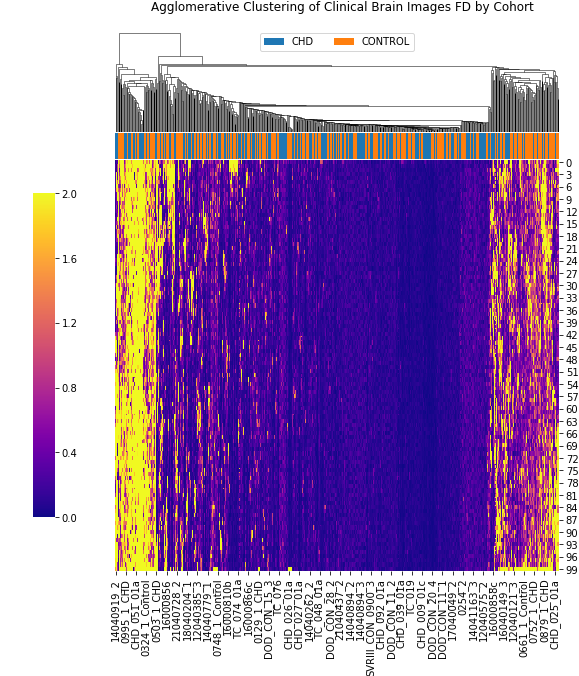
\includegraphics[width=1.0\textwidth]{6/figures/cohort-bold-fd-sns-agg.png}
		\caption{FD}
	\end{subfigure}
	\begin{subfigure}{0.49\textwidth}
		\centering
		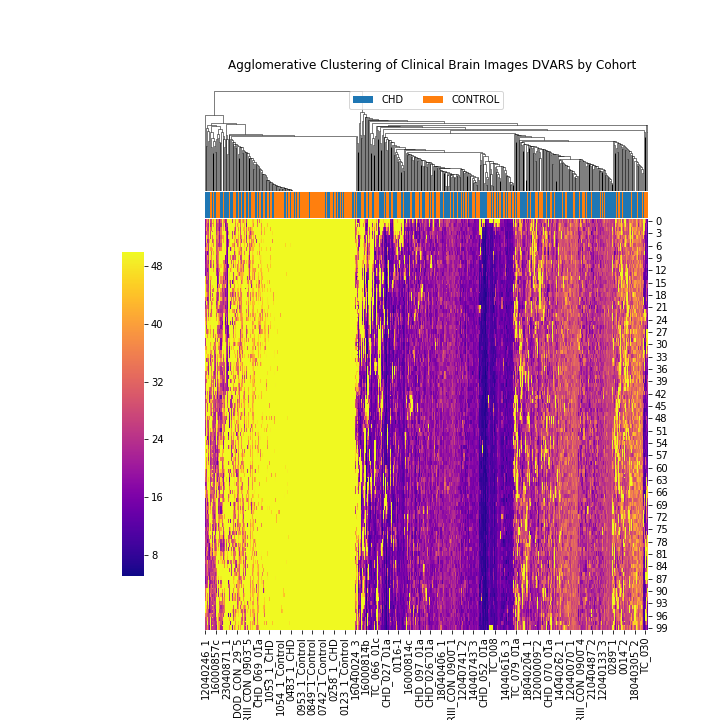
\includegraphics[width=1.0\textwidth]{6/figures/cohort-bold-dvars-sns-agg.png}
		\caption{DVARS}
	\end{subfigure}
	
	\begin{subfigure}{0.49\textwidth}
		\centering
		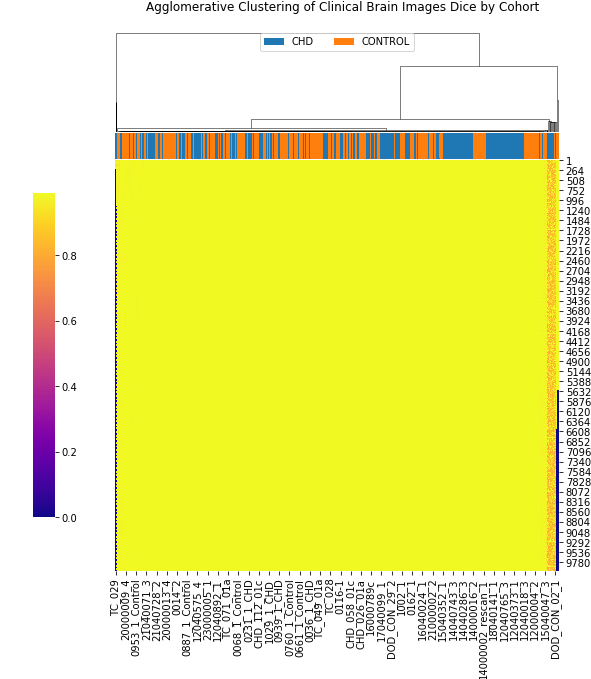
\includegraphics[width=1.0\textwidth]{6/figures/cohort-bold-dice-sns-agg.png}
		\caption{Dice}
	\end{subfigure}
	\begin{subfigure}{0.49\textwidth}
		\centering
		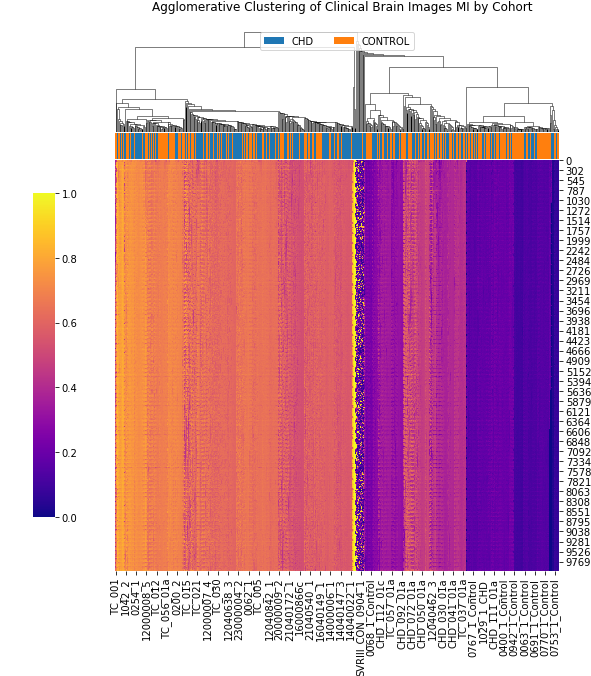
\includegraphics[width=1.0\textwidth]{6/figures/cohort-bold-mi-sns-agg.png}
		\caption{MI}
	\end{subfigure}
\vspace{-10mm}
\caption{The original preadolescent, neonatal, and fetal images clustered by each metric using agglomerative clustering and labeled by disease status.}
\label{fig:mocha-cohorts-sns-agg}
\end{figure}

The FD, DVARS, Dice matrices, and MI matrices for the original clinical brain images were projected into 2D space and labeled using each subject's disease status. The projections of this data can be seen in Figure \ref{fig:mocha-ages-data-2d}. In this figure, each column represents a different dimensionality reduction technique, and each row represents a different metric type. The different dimensionality reduction techniques offer different views on the same data, though the relationships between these views are not always clear. It is very difficult to see any distinct groups of CHD or control labels in any of these views.

The FD, DVARS, Dice matrices, and MI matrices were then each clustered using agglomerative clustering. Heatmaps of these clustering results can be seen in Figure \ref{fig:mocha-cohorts-sns-agg}. The columns of the heatmaps show the feature vectors used to represent each image sequence. The colorbars to the left of the heatmaps show the range of values present in each heatmap. In all four heatmaps, darker colors represent lower values. At the top of each heatmap is a row of colored labels where the blue labels indicate subjects who have CHD and the orange labels indicate control subjects. Above the row of labels is a dendrogram. The dendrogram explicitly shows the distances between the feature vectors. Each vertical bar in a dendrogram represents the distance between that feature vector and the feature vector or group of feature vectors most similar to it. The horizontal bars indicate connections between feature vectors or groups of feature vectors which are the next closest to each other.

The heatmaps for the clustering results generated using the FD, DVARS, and MI metrics each show several distinct vertical bands representing clusters of similar feature vectors. The heatmap for the Dice metrics is less interpretable as most of the values in the heatmap are close to 1.0. In all four sets of clustering results, there are no distinguishable clusters which are mostly composed of either CHD or control subjects.

\subsection{Age Groups}

\begin{figure}
\centering
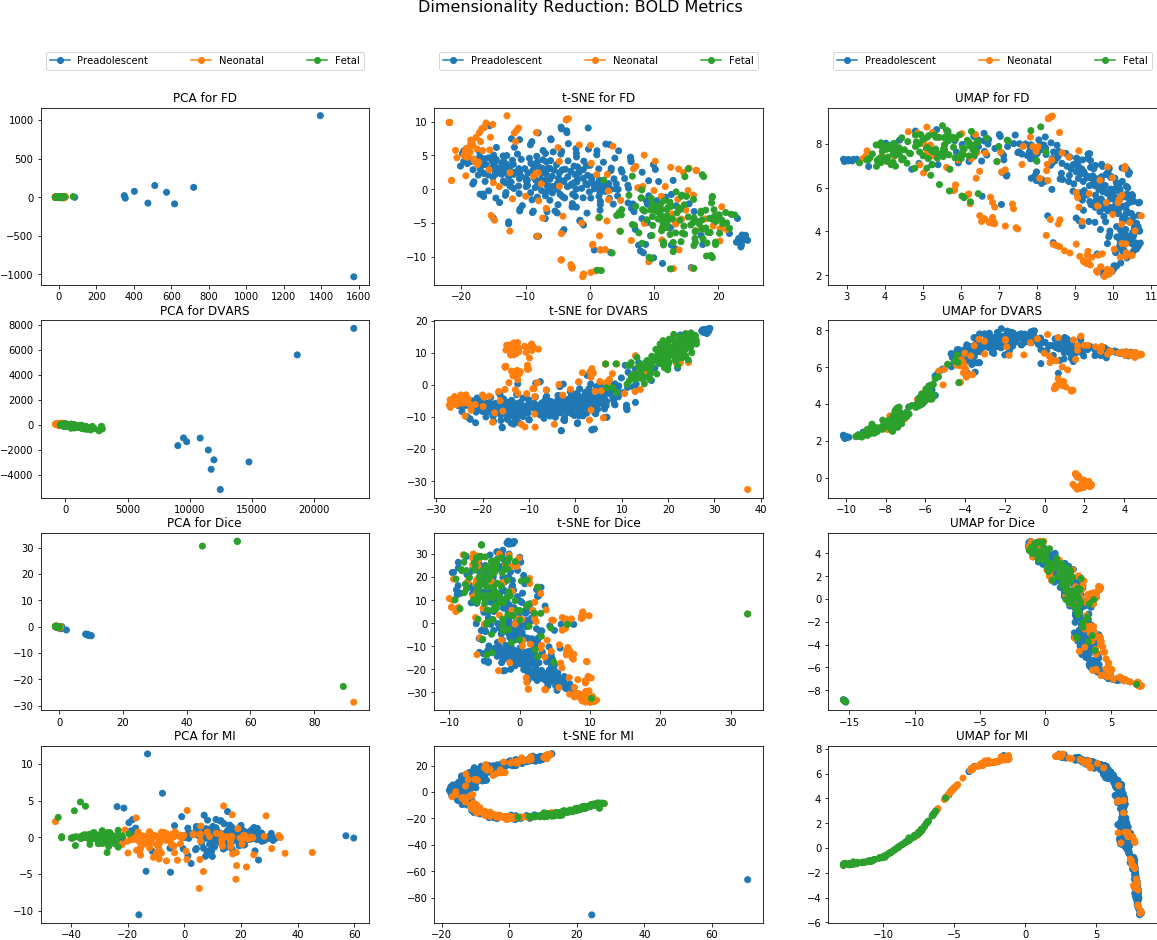
\includegraphics[width=1.0\textwidth]{6/figures/bold-2d-all-agegroup.png}
\caption{The data for the four metrics used to evaluate motion in the clinical brain images projected using different methods into 2D space and labeled by age group.}
\label{fig:mocha-ages-data-2d}
\end{figure}

\begin{figure}[]
	\centering
	\begin{subfigure}{0.49\textwidth}
		\centering
		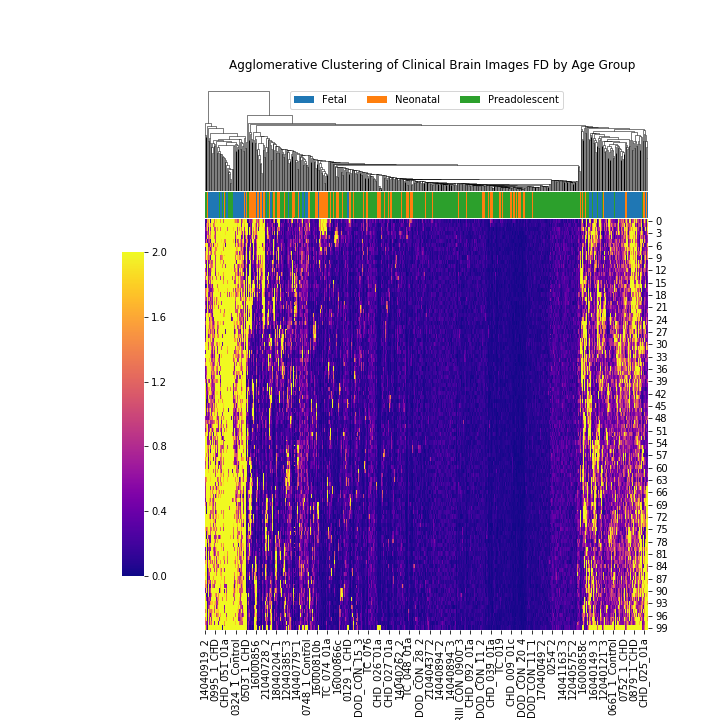
\includegraphics[width=1.0\textwidth]{6/figures/agegroup-bold-fd-sns-agg.png}
		\caption{FD}
	\end{subfigure}
	\begin{subfigure}{0.49\textwidth}
		\centering
		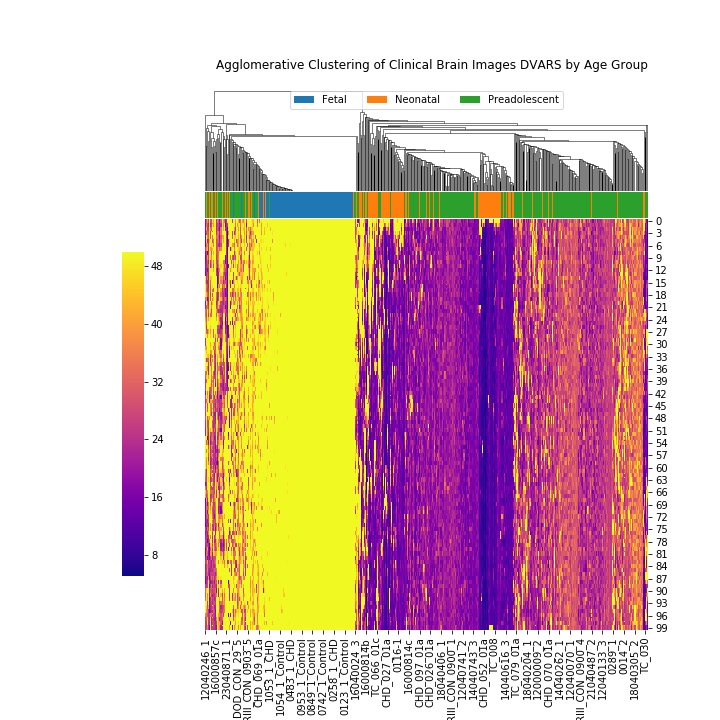
\includegraphics[width=1.0\textwidth]{6/figures/agegroup-bold-dvars-sns-agg.png}
		\caption{DVARS}
	\end{subfigure}
	
	\begin{subfigure}{0.49\textwidth}
		\centering
		\includegraphics[width=1.0\textwidth]{6/figures/agegroup-bold-dice-sns-agg.png}
		\caption{Dice}
	\end{subfigure}
	\begin{subfigure}{0.49\textwidth}
		\centering
		\includegraphics[width=1.0\textwidth]{6/figures/agegroup-bold-mi-sns-agg.png}
		\caption{MI}
	\end{subfigure}
\vspace{-10mm}
\caption{The preadolescent, neonatal, and fetal images clustered by each metric using agglomerative clustering and labeled by age group.}
\label{fig:mocha-ages-sns-agg}
\end{figure}

The three age groups of interest were preadolescent, neonatal, and fetal. Figure \ref{fig:mocha-ages-data-2d} shows the motion metrics projected into 2D and labeled with the correct age groups. The blue labels indicate preadolescent subjects, the orange labels indicate neonatal subjects, and the green labels indicate fetal subjects. In this figure, the first three rows of the first column (PCA of FD, DVARS, and Dice) show highly concentrated groups of subjects with some sparse, distant outliers. In the first three rows of the second and third columns (t-SNE and UMAP for FD, DVARS, and Dice), the preadolescent and fetal groups are mostly separate, and the neonatal subjects span these groups. In the last row of all three columns (PCA, t-SNE, and UMAP for MI), groups of subjects from the different age groups are clearly visible despite some overlap. 

The four types of metrics were clustered using agglomerative clustering. The agglomerative clustering results labeled using the age groups can be seen in Figure \ref{fig:mocha-ages-sns-agg}. The same clusters present in the heatmaps of Figure \ref{fig:mocha-cohorts-sns-agg} can be seen in these heatmaps, but the age group labels are more clearly related to the clusters in the DVARS and MI heatmaps.

In the heatmap for clustering performed with DVARS feature vectors, the brightest uniform band mostly consists of fetal subjects. The darker, more variable band next to the group of fetal subjects is primarily composed of neonatal subjects. Groups of preadolescent subjects can also be easily identified. 

Clusters of subjects from the same age group can also be clearly identified in the heatmap for the MI feature vectors. The bright, wide vertical band encompassing the left half of the heatmap consists of subjects mostly from the preadolescent cohort. The darkest vertical bands on the right of the heatmap are made of almost exclusively fetal subjects. The clusters between the preadolescent group and the neonatal group comprise the neonatal subjects and some preadolescent subjects. 

\begin{figure}
\centering
\includegraphics[width=1.0\textwidth]{6/figures/bold-mi-agegroup.png}
\caption{The results of clustering the clinical images using the MI matrices and the age group labels.}
\label{fig:mocha-ages-mi-bold}
\end{figure}

The MI feature vectors were used to perform k-means clustering and spectral clustering in addition to the agglomerative clustering. Figure \ref{fig:mocha-ages-mi-bold} shows a grid of scatter plots of the original data and the clustering results. The feature vectors in the first column are labeled with the true age group labels of the data. The vectors in the second, third, and fourth columns are labeled using the labels produced by k-means, spectral, and agglomerative clustering, respectively, where the number of clusters is three. 

\begin{figure}
\centering
\includegraphics[width=0.9\textwidth]{6/figures/spectral-revised.png}
\caption{Iteratively removing clusters containing less than 10\% of the data in the data set and repeating the spectral clustering process produced meaningful clusters similar to those produced by the k-means and agglomerative methods.}
\label{fig:spectral-revised}
\end{figure}

Initially, the spectral clustering results essentially identified a pair of outliers in the data set. The outliers were removed and the clustering was redone, but another pair of outliers was identified in this second iteration. We performed several iterations of identifying data belonging to outlier clusters, which we defined as clusters containing less than 10\% of the total data in the data set, and repeating the clustering. This process reduced the number of samples in the data set from 564 to 545 but did produce meaningful clusters. The results of spectral clustering the reduced data set can be seen in Figure \ref{fig:spectral-revised}. 

\begin{table}[]
\centering
\caption{The composition of age groups in each cluster produced using the MI feature vectors and k-means clustering.}
\label{tab:mocha-mi-kmeans}
\begin{tabular}{|l|c|c|c|}
\hline
\textbf{Label} & \multicolumn{1}{l|}{\textbf{Cluster 1}} & \multicolumn{1}{l|}{\textbf{Cluster 2}} & \multicolumn{1}{l|}{\textbf{Cluster 3}} \\ \hline
\textbf{Preadolescent} & 271 & 3   & 28  \\ \hline
\textbf{Neonatal}      & 45  & 8   & 86  \\ \hline
\textbf{Fetal}         & 0   & 122 & 1   \\ \hline
\textbf{Total}         & 316 & 133 & 115 \\ \hline
\end{tabular}
\end{table}

\begin{table}[]
\centering
\caption{The composition of age groups in each cluster produced using the MI feature vectors and spectral clustering.}
\label{tab:mocha-mi-spectral}
\begin{tabular}{|l|c|c|c|}
\hline
\textbf{Label} & \multicolumn{1}{l|}{\textbf{Cluster 1}} & \multicolumn{1}{l|}{\textbf{Cluster 2}} & \multicolumn{1}{l|}{\textbf{Cluster 3}} \\ \hline
\textbf{Preadolescent} &   4 & 278 &  9 \\ \hline
\textbf{Neonatal}      &   6 &  55 & 76 \\ \hline
\textbf{Fetal}         & 116 &   0 &  1 \\ \hline
\textbf{Total}         & 126 & 333 & 86 \\ \hline
\end{tabular}
\end{table}

\begin{table}[]
\centering
\caption{The composition of age groups in each cluster produced using the MI feature vectors and agglomerative clustering.}
\label{tab:mocha-mi-agg}
\begin{tabular}{|l|c|c|c|}
\hline
\textbf{Label} & \multicolumn{1}{l|}{\textbf{Cluster 1}} & \multicolumn{1}{l|}{\textbf{Cluster 2}} & \multicolumn{1}{l|}{\textbf{Cluster 3}} \\ \hline
\textbf{Preadolescent} & 282 & 19 & 1   \\ \hline
\textbf{Neonatal}      & 58  & 76 & 5   \\ \hline
\textbf{Fetal}         & 0   & 1  & 122 \\ \hline
\textbf{Total}         & 340 & 96 & 128 \\ \hline
\end{tabular}
\end{table}

The composition of the clusters produced by each type of clustering can be seen in Tables \ref{tab:mocha-mi-kmeans}, \ref{tab:mocha-mi-spectral}, and \ref{tab:mocha-mi-agg}. The frequency counts in Tables \ref{tab:mocha-mi-kmeans} and \ref{tab:mocha-mi-agg} were comparable despite the different clustering methods. The contents of table \ref{tab:mocha-mi-spectral} were calculated using the reduced set of data that produced interpretable (non-outlier based) clustering results. These results mirror those in Tables \ref{tab:mocha-mi-kmeans} and \ref{tab:mocha-mi-agg}. The results of our cluster analysis suggest that there are detectable differences in the rs-fMRIs of different age groups of patients from different age groups.

\section{Summary}

In this chapter, we compared the rs-fMRIs before and after registration for the simulated and clinical images. These comparisons were performed using four metrics: FD, DVARS, Dice, and MI. The FD and DVARS metrics showed that both registration types had statistically significant impacts on these metrics at the population level. These impacts varied between populations. The Dice and MI metrics were used to compare all volumes in a single sequence to each other. These metrics demonstrated the impact of volume registration on the image sequences as a whole. 

The motion patterns of the original image sequences characterized by the four metrics were used to characterize motion in the clinical brain images. No clear relationship between motion and disease status was found, but clustering showed a relationship between motion and age group.







